\section{Background estimation}
%%%%%%%%%%%%%%%%%%%%%%%%%%%%%%%%%%%%%%%%%%%%%%%%%%%%%%%%%%%%%%%%%%%%%%
\label{sec:Backgrounds}


\subsection{Top quark background \label{sec:TTBackground}}

In this analysis the top quark background is divided into two different categories depending on the number of jets in the event. In the two categories different selections are applied, especially concerning the b-tagging requirements.

The general strategy for determining the residual top events in the signal region is to first measure the top tagging efficiencies from an orthogonal region of phase space in data. The orthogonal phase space is  defined inverting the b-veto requirement of the signal region, in such a way to have a control region enriched in top quark events.  Then, using this efficiency, the number of events with the associated uncertainty is propagated from the control region to the signal region.
The number of surviving top events in the signal region would then be:

\begin{equation}
 N^{\mathrm{signal}}_{bveto} = N^{\mathrm{control}}_{btag} \cdot \frac{1-\epsilon_{\mathrm{top}}}{\epsilon_{\mathrm{top}}}
\label{eq:top_equation}
\end{equation}

where $N^{\rm control}_{\rm btag}$ is the number of events in the 
control region and $\epsilon_{\rm top}$ is the efficiency as measured
in data.

The methods to estimate the top background contribution in the two jet categories are different and are explained below.


\subsubsection{0-jets category}
Most of the top background, composed of \ttbar and tW processes, is rejected in the 0-jet bin by the
jet veto. The top-tagging efficiency in the zero jet bin, $\epsilon_{\rm tag}^{0-jet}$, is the probability for a top event to
fail one of either the b-tagging veto or the soft muon veto, and is defined as:

\begin{equation}\label{eq:eff_top_0j}
\epsilon_{\rm tag} = \frac{N_{\rm tag}^{\rm control}}{N^{\rm control}} \quad ,
\end{equation}

where $N^{\rm control}$ is the number of events in the top control phase space defined requiring one b-tagged jet with $\pt>30$\GeV, and $N_{\rm tag}^{\rm control}$ is the subset of those events that pass either the soft muon tagging or the low-\pt b jet tagging. The purity of this control sample, as estimated from simulation, is about 97\%. The remaining 3\% background contribution is estimated from simulation and subtracted from the numerator and denominator of Eq.~\eqref{eq:eff_top_0j}. The efficiency $\epsilon_{\rm top}^{0-jet}$ can then be estimated using the following formula:

\begin{equation}\label{eq:eff_top_0j}
\epsilon_{\rm top}^{0-jet} = f_{\ttbar} \cdot \epsilon_{2b} + f_{tW} \cdot ( x \cdot \epsilon_{2b} + (1-x) \cdot \epsilon_{\rm tag} ) \quad ,
\end{equation}

\begin{equation}
\epsilon_{2b} = 1 - (1 - \epsilon_{\rm tag})^{2} \quad ,
\end{equation}
where $f_{\ttbar}$ and $f_{tW}$ are the \ttbar and tW fractions respectively, $x$ is the fraction of tW events containing 2 b jets, and $\epsilon_{2b}$ is the efficiency for a top event with 0 counted jets, i.e. two soft b jets, to pass the top veto. For the ratio of \ttbar and tW cross-sections an uncertainty of 17\% is assumed. The fraction $f_{\ttbar}$ is estimated using MC simulation of the \ttbar and tW processes at NLO accuracy.

Using this procedure a data/simulation scale factor of $0.98 \pm 0.17$ is found, and is applied to correct the MC simulation in order to match the data.



\subsubsection{Category with more than 0 jets}
The strategy for the estimation of the top background in events with at least one jet with $\pt$ greater than 30 \GeV is the following. First of all the efficiency for tagging a b jet is measured both in data and simulation and the values are used to correct the simulation for different b-tagging efficiencies in data and simulation. This evaluation is performed in a control region, called CtrlTP, containing at least two jets, using a Tag\&Probe technique. The procedure to extract these scale factors is presented in Sec.~\ref{sec:TagAndProbe}. Then a larger statistics control region, CtrlDD, is defined by requiring at least one b-tagged jet and we use the simulation, corrected for the previously computed b-tagging efficiency scale factor, to derive the factor that connects the number of events in CtrlDD to the number of events in the signal region. This second step is explained in detail in Sec.~\ref{sec:DD}. 

\subsubsection{Tag\&Probe \label{sec:TagAndProbe}}
The Tag\&Probe technique is a method to estimate the efficiency of a selection on data. In can be applied whenever one has two objects in one event, by using one of the two, the \tg{}, to identify the process of interest, and using the second, the \probe{}, to actually measure the efficiency of the selection being studied. In our case we want to measure the b-tagging efficiency, so what we need is a sample with two b-jets per event. The easiest way to construct such a sample is to select $t\bar{t}$ events.

The CrtlTP control region is defined selecting the events which pass the lepton preselection cuts listed in Sec.~\ref{subsec:EventSelection}, and have at least two jets with \pt greater than 30 \GeV.
One of the two leading jets is required to have a \jpb score higher than 0.5. From events in this control region we built \tp{} pairs as follows. For each event the two leading jets are considered. If the leading jet passes the \jpb cut of 0.5, that is considered a \tg{}, and the sub-leading jet is the \probe{}. In order to avoid any bias that could arise from the probe being always the second jet, the pair is tested also in reverse order, meaning that the sub-leading jet is tested against the \tg{} selection, and in case it passes, then the leading jet is used as \probe{} in an independent \tp{} pair. This means that from each event passing the CrtlTP cuts one can build up to two \tp{} pairs. 

If the \tg{} selection were sufficient to suppress any non top events, one could estimate the efficiency by dividing the number of \tp{} pairs in which the \probe{} passes the analysis cut \jpb$>$1.4 (\tpp) by the total number of \tp{} pairs. However this is not the case. 
In order to estimate the efficiency in the presence of background a variable that discriminates between true b-jets and other jets in a $t\bar{t}$ sample is chosen. The variable is the \pt of the \probe{} jet. For real b-jets this variable has a peak around 60 \GeV, while it does not peak for other jets. The idea is to fit simultaneously the \pt spectrum for \probe{} jets in \tpp{} and \tfp{} pairs, linking together the normalizations of the two samples as follows:
\begin{equation}
N_{TPP}=N_{s}\epsilon_{s} + N_b\epsilon_{b}
\end{equation}
\begin{equation}
N_{TFP}=N_{s}(1-\epsilon_{s}) + N_b(1-\epsilon_{b})
\end{equation}
where $N_{\rm TPP}$ is the number of \tpp{} pairs, $N_{\rm TFP}$ is the number of \tfp{} pairs, $N_{\rm s}$ is the number of \tp{} pairs in which the probe is a b-jet, $N_{\rm b}$ is the number of \tp{} pairs in which the probe is a not b-jet, $\epsilon_{\rm s}$ is the b-tagging efficiency, $\epsilon_{\rm b}$ is the probability of identifying as b-jet a non-b-jets, i.e. the mistag rate. 

A $\chi^{2}$ simultaneous fit of the \probe{} \pt spectrum for \tpp{} and \tfp{} pairs is performed, deriving the shapes for true b-jets and non-b-jets from the simulation, and extracting $N_{\rm s}$, $N_{\rm b}$, $\epsilon_{\rm s}$ and $\epsilon_{\rm b}$ from the fit.
The result of the fit on simulation is shown in Fig.~\ref{fig:mc_tp}. The relevant efficiencies are:
\begin{equation}
\epsilon_{s}^{MC}=0.7663\pm0.0072
\end{equation}
\begin{equation}
\epsilon_{b}^{MC}=0.208\pm0.015
\end{equation}
We have checked that these values are consistent with the true value for the b-tagging efficiency. The true value is computed by selecting jets that are matched within a cone of $\Delta{R}<0.5$ with a generator level b-quark, and counting the faction of those that pass the \jpb cut of 1.4. This means that the \tp{} method does not introduce biases within the simulation statistic accuracy.

\begin{figure}[b]
\centering
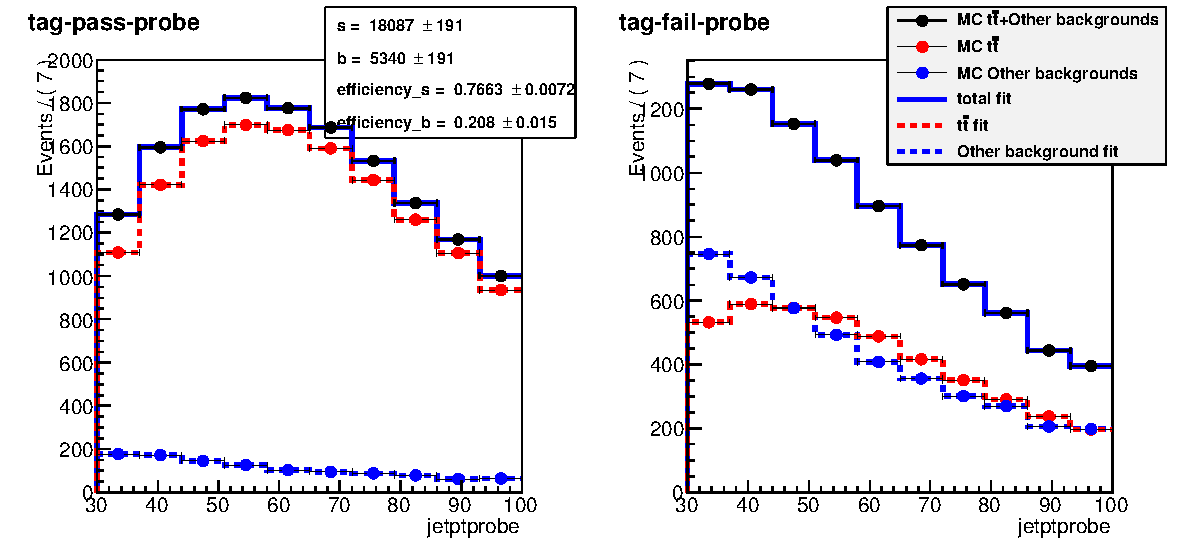
\includegraphics[width=0.8\textwidth]{images/mc_pt_probe.pdf}
\caption{Simultaneous fit of the \tpp{} and \tfp{} pairs in the MC.\label{fig:mc_tp}}
\end{figure}

In order to assess the robustness of the fit, 5000 toy MC samples have been generated with a statistics equivalent to the one expected in data and the same fit is performed. All the 5000 fit succeeded, and the pull distributions for $\epsilon_{\rm s}$ and $\epsilon_{\rm b}$ parameters are shown in Fig.~\ref{fig:pullstp}. The plots show the pull of the efficiencies measured in the fit, where the pull variable for each toy $i$ is defined as:

\begin{equation}
pull(\epsilon_{\rm s (b)}) = \frac{\epsilon_{\rm s (b)}^{\rm true} - \epsilon_{\rm s (b)}^{i}}{\sigma(\epsilon_{\rm s (b)}^{i})}
\end{equation}

The pulls are centered on 0 and have $\sigma$ close to 1, as expected.

\begin{figure}[t]
\centering
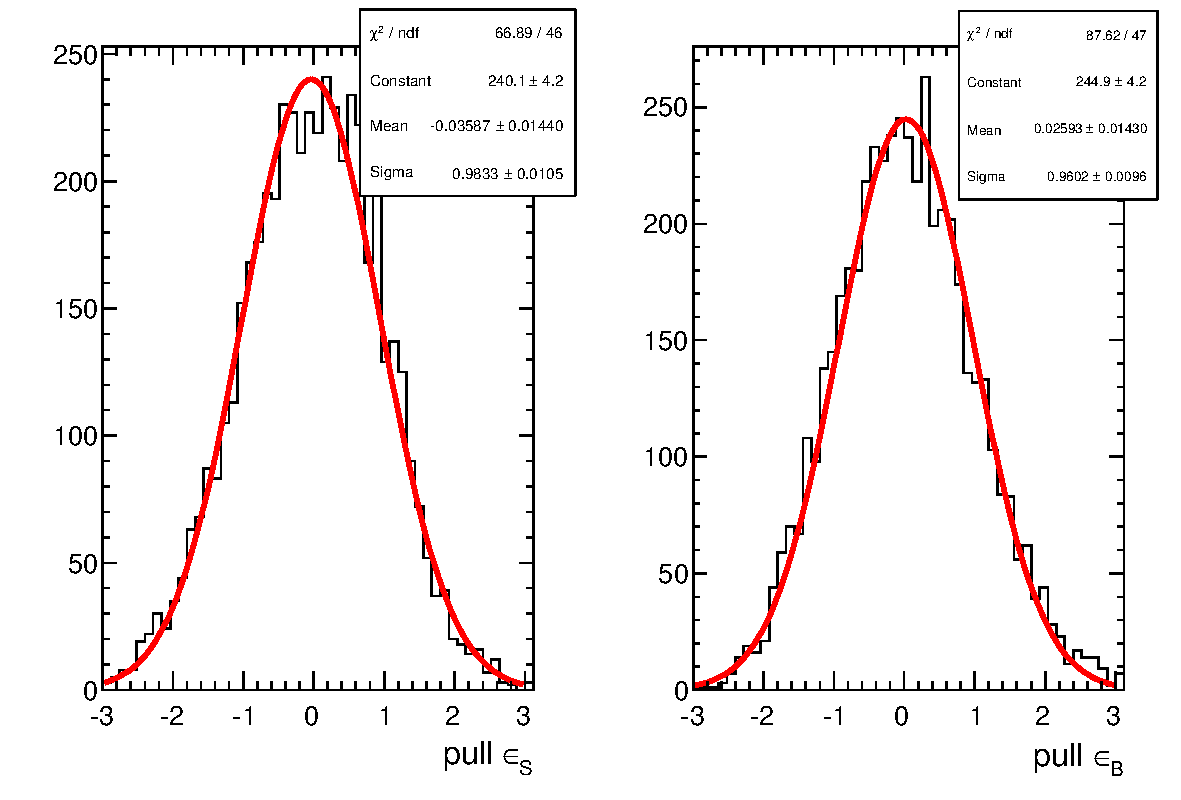
\includegraphics[width=0.8\textwidth]{images/pulls_mc.pdf}
\caption{Pulls of the $\epsilon_{s}$ and $\epsilon_{b}$ parameters in 5000 toy MC.\label{fig:pullstp}}
\end{figure}
An example fit for one of the toys is shown in  Fig.~\ref{fig:toy_tp}
\begin{figure}[b]
\centering
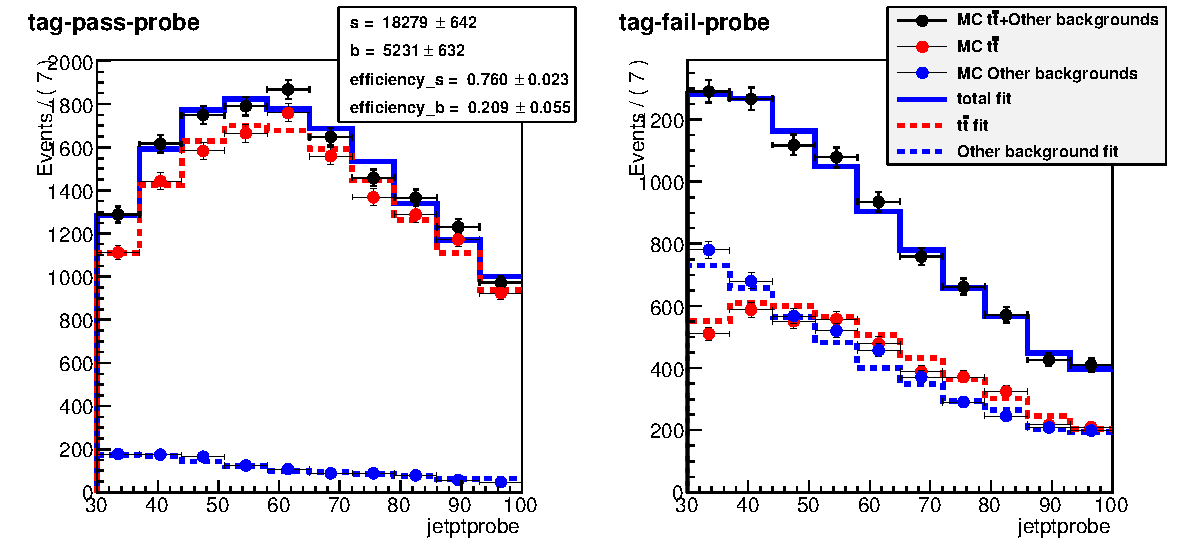
\includegraphics[width=0.8\textwidth]{images/mc_pt_probe_toy.pdf}
\caption{Fit of a toy MC sample.\label{fig:toy_tp}}
\end{figure}

Before running the fit on data, the shapes used in the fit have been validated. To do so, a purer top enriched phase space has been defined by requiring exactly two jets with \jpb score higher than 1.5 and no additional b-tagged jets, rejecting also jets with \pt smaller than 30 \GeV. On this purer sample we have compared data against the shape used to fit the true b-jets in the \tpp{} distribution. The result is shown in Fig.~\ref{fig:purett} and shows good agreement.
\begin{figure}[t]
\centering
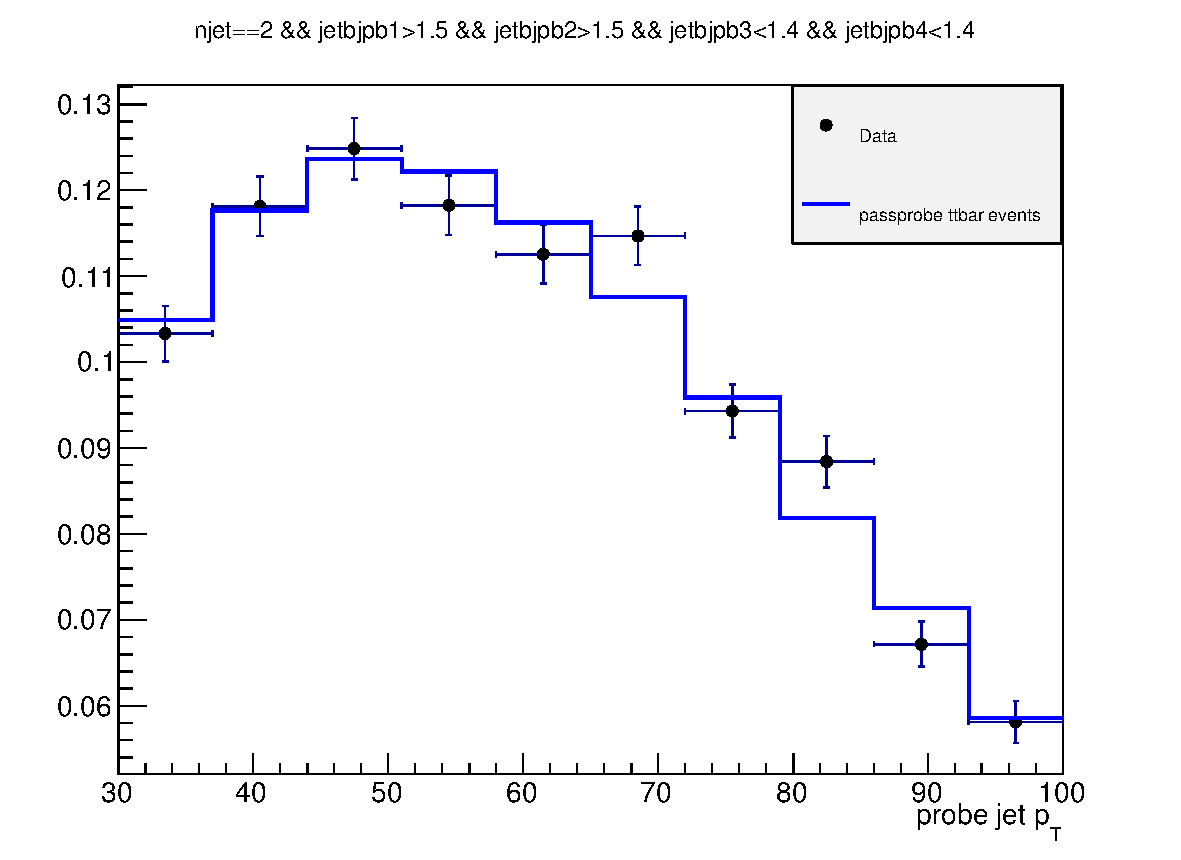
\includegraphics[width=0.6\textwidth]{images/passprobe_data_mc.pdf}
\caption{Shape comparison for the \probe{} \pt spectrum in data and in MC in a very pure \ttbar sample.\label{fig:purett}}
\end{figure}

Finally the fit has been performed on data, as shown in Fig.~\ref{fig:data_tp}, providing the following efficiencies:
\begin{equation}
\epsilon_{s}^{Data}=0.769\pm0.022
\end{equation}
\begin{equation}
\epsilon_{b}^{Data}=0.121\pm0.054
\end{equation}

\begin{figure}[b]
\centering
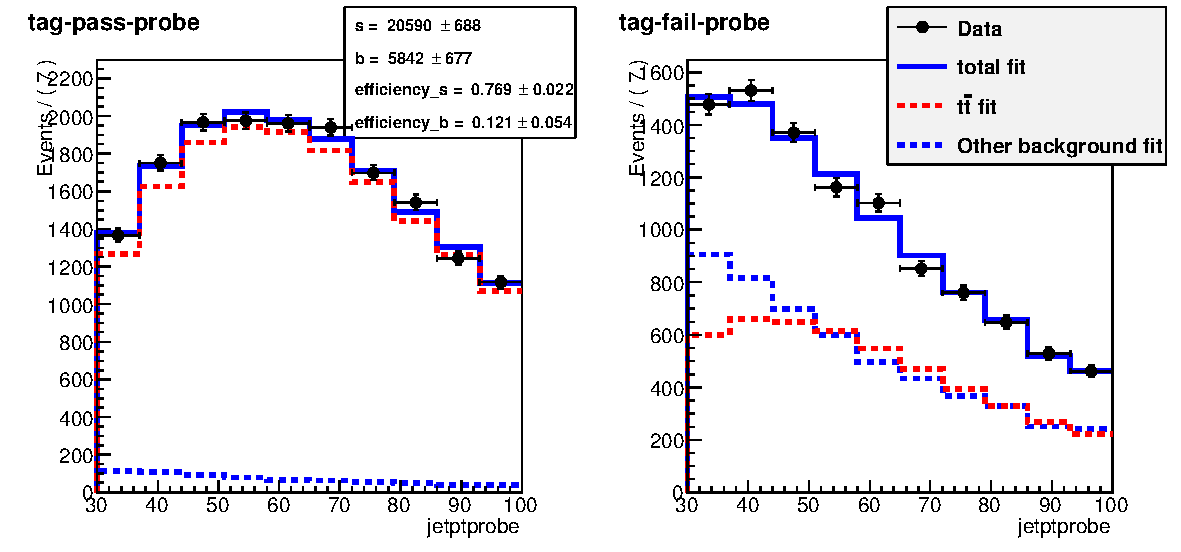
\includegraphics[width=0.8\textwidth]{images/data_ptprobe.pdf}
\caption{Simultaneous fit of the \tpp{} and \tfp{} pairs in data.\label{fig:data_tp}}
\end{figure}

Further studies have been performed to assess the effect of the relative uncertainty on the \ttbar and tW event fractions. The same procedure described above has been applied to different simulation templates obtained varying the \ttbar and tW fractions within theoretical uncertainties, and the effect on the parameters extracted with the fit procedure is found to be well below the fit uncertainties.


\subsubsection{Data driven estimation \label{sec:DD}}
In addition to the b-tagging efficiency, the other ingredient to estimate the \ttbar background is the process cross section. The idea is to measure the cross section in a \ttbar enriched control region, that is called CtrlDD. CtrlDD is defined according to the lepton preselection cuts defined in Sec.~\ref{sec:Selections}, and requiring in addition at least one jet with \jpb score higher than 1.4.

From the simulation we derive the factor $\alpha$ that connects CrtlDD to the signal region, calculating the ratio of \ttbar events in the two regions:

\begin{equation}
\alpha=\frac{N_{\ttbar~MC}^{SIG}}{N_{\ttbar~MC}^{CtrlDD}} \quad.
\end{equation}

The number of events in the CtrlDD region in data is counted, subtracting the expected number of events from non-\ttbar backgrounds, and obtaining $N_{\ttbar~Data}^{CtrlDD}$. Finally the number of expected \ttbar events in the signal region ($N_{\ttbar~Data}^{SIG}$) is obtained as:

\begin{equation}
N_{\ttbar~Data}^{SIG} = \alpha{}N_{\ttbar~Data}^{CtrlDD}.
\end{equation}

In evaluating $\alpha$ and its error the b-tagging efficiencies determined in Sec.~\ref{sec:TagAndProbe} are used. 
For each event an efficiency scale factor and a mistag rate scale factor are derived, depending on whether the event falls in the signal or CtrlDD region.

\begin{equation}
\label{eq:sfsig}
SF_{SIG} = \left(\frac{1-\epsilon_{s}^{Data}}{1-\epsilon_{s}^{MC}}\right)^{min(2, n_{b-jets})} \left(\frac{1-\epsilon_{b}^{Data}}{1-\epsilon_{b}^{MC}}\right)^{n_{non-b-jets}} 
\end{equation}

\begin{equation}
\label{eq:sfbkg}
SF_{CtrlDD} = \left(\frac{\epsilon_{s}^{Data}}{\epsilon_{s}^{MC}}\right)^{(jet1 == b-jet)} \left(\frac{\epsilon_{b}^{Data}}{\epsilon_{b}^{MC}}\right)^{(jet1 == non-b-jets)} 
\end{equation}

where $n_{b-jets}$ is the number of true b-jets in the event and $n_{non-b-jets}$ is the number of non-b-jets in the event. The writing $jet1 == b-jet$ ($jet1 == non-b-jets$) is a boolean flag that is true when the leading jet, the one used for the CtrlDD selection, is (not) a true b-jet.

Since the efficiency and mistag rate that have been measured on data are close to the one in the simulation, it was decided to assume a scale factor of 1 for both b-tagging efficiency and mis-tag rate. This means that the central values of the scale factors defined in Eq.~\ref{eq:sfsig} and Eq.~\ref{eq:sfbkg} is 1, but these numbers have an error that is derived assuming an uncertainty on $\epsilon_{s}^{Data}$ and $\epsilon_{b}^{Data}$ that covers both the statistical error from the fit of the two quantities and the difference with respect to the simulation.
This results in an up and a down variation of the scale factors in the signal and CtrlDD regions, that is used to derive an error on $\alpha$.

A data driven estimation of the top quark background with the method described above is performed in each of the \pth bins independently. The reason to make this estimation in $\pth$ bins, rather than inclusively is explained in Fig.~\ref{fig:ttpth}, where the \pth distribution is shown in the CtrlDD region normalized to the cross section measured by a specific CMS analysis~\cite{Khachatryan:2016mqs}. As shown in the ratio plot, an overall normalization factor would not be able to accommodate for the variations of the data/simulation ratio from bin to bin.

\begin{figure}[b]
\centering
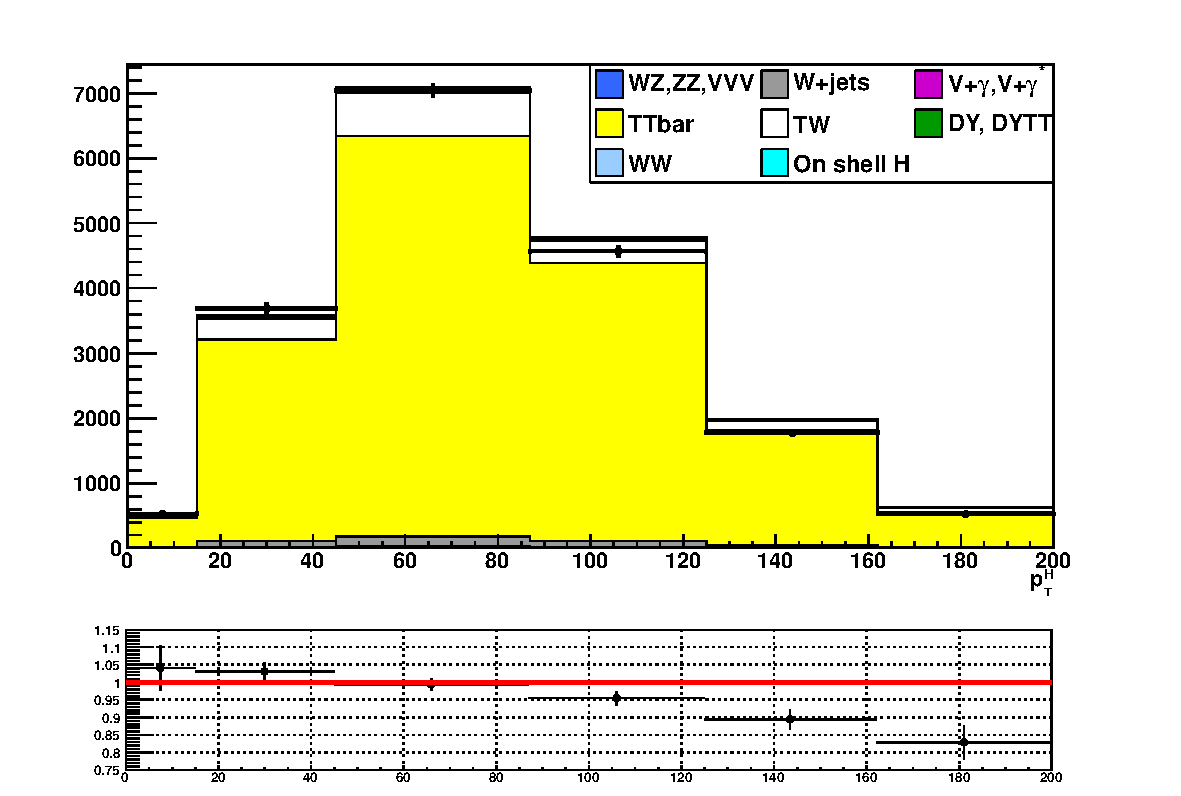
\includegraphics[width=0.6\textwidth]{images/ttpth.pdf}
\caption{$\pth$ distribution in the CtrlDD control region.\label{fig:ttpth}}
\end{figure}

The $\alpha$ factors for each bin and the number of events in signal, CtrlDD regions in MC as well as in data are listed in Tab.~\ref{tab:ttdd}.
\begin{table}
\centering
\begin{tabular}{c c c c c c}
\hline
\pth [\GeV] & $N_{CTRL}^{DATA}$ & $N_{CTRL}^{TOP}$ &  $N_{SIG}^{TOP}$ &
$\alpha$ & $\Delta\alpha$ \\ 
\hline\hline
$[0 \textendash 15]$ & 406.71 & 358.78 & 117.83 & 0.328 & 0.075 \\ 
$[15 \textendash 45]$ & 2930.14 & 2703.44 & 859.08 & 0.318 & 0.071 \\ 
$[45 \textendash 85]$ & 5481.02 & 5207.48 & 1506.05 & 0.289 & 0.065 \\ 
$[85 \textendash 125]$ & 4126.35 & 4032.56 & 861.22 & 0.214 & 0.052 \\ 
$[125 \textendash 165]$ & 1612.64 & 1654.27 & 304.69 & 0.184 & 0.055 \\ 
$[165 \textendash \infty]$ & 647.50 & 760.37 & 201.70 & 0.265 & 0.147 \\ 
\hline
\end{tabular}
\caption{Data driven scale factors related to the top quark background estimation.\label{tab:ttdd}}
\end{table}

A comparison of the $\mll$ distribution in the six $\pth$ bins used in the analysis in CtrlDD after the data driven correction is shown in Fig.~\ref{fig:mllCtrlDD}
\begin{figure}[htb]
\centering
\subfigure[$\pth<15\GeV$]{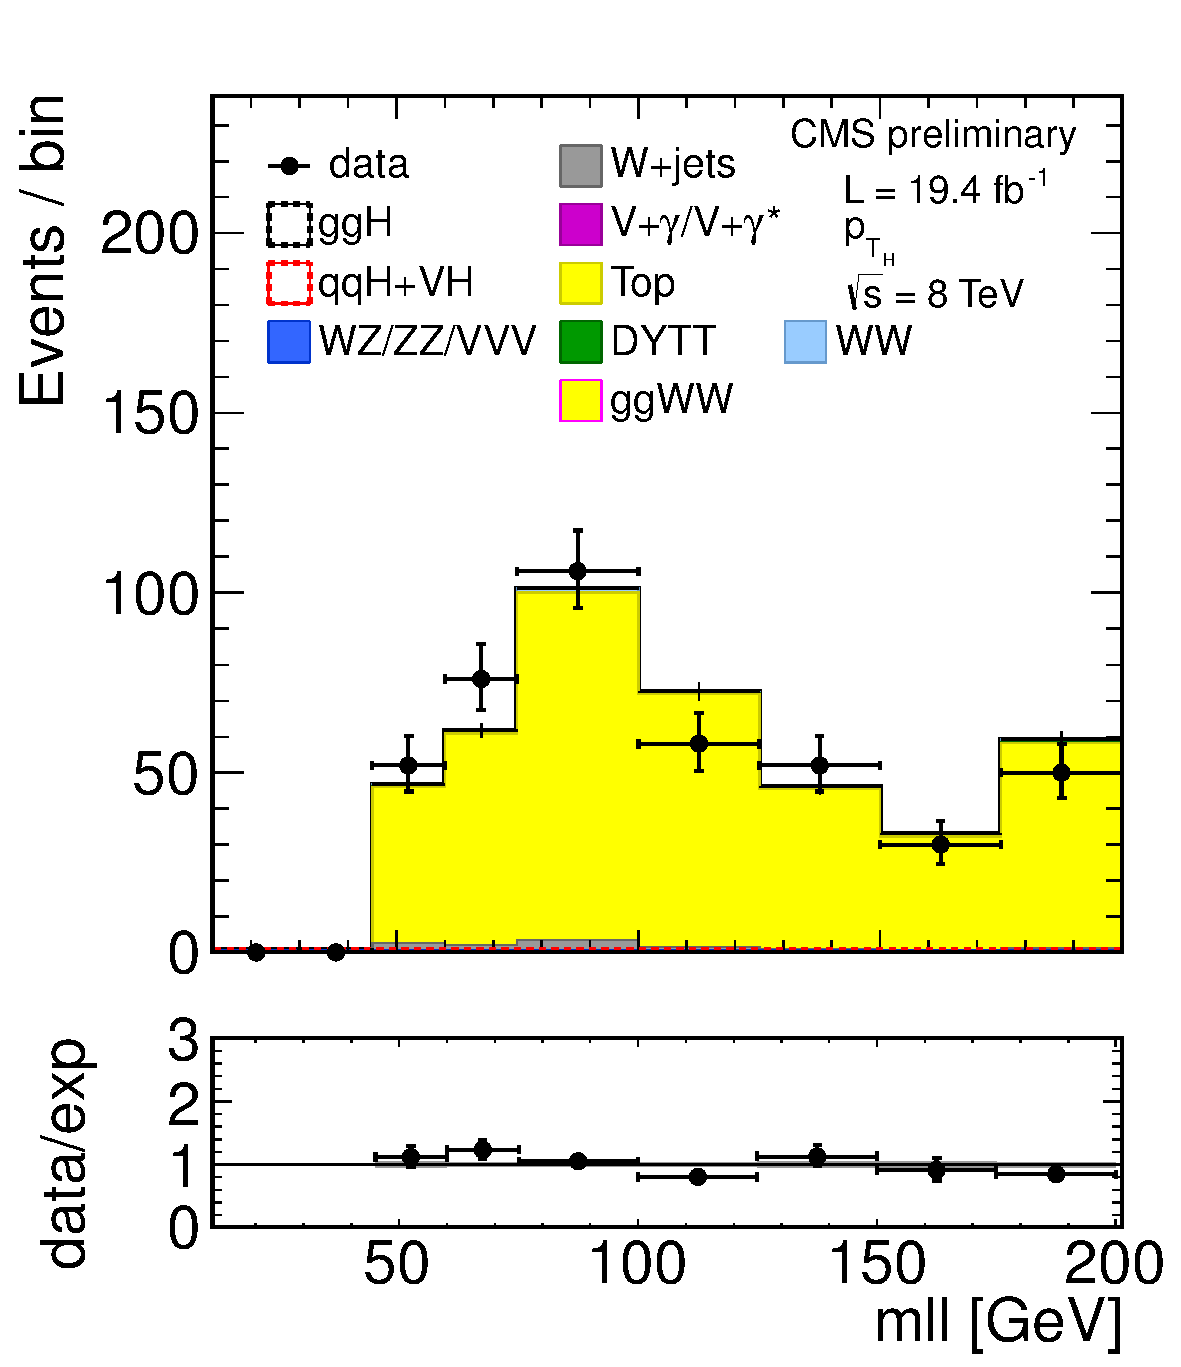
\includegraphics[width=0.35\textwidth]{images/mllBin0CtrlDD.pdf}}
\subfigure[$15\GeV<\pth<45\GeV$]{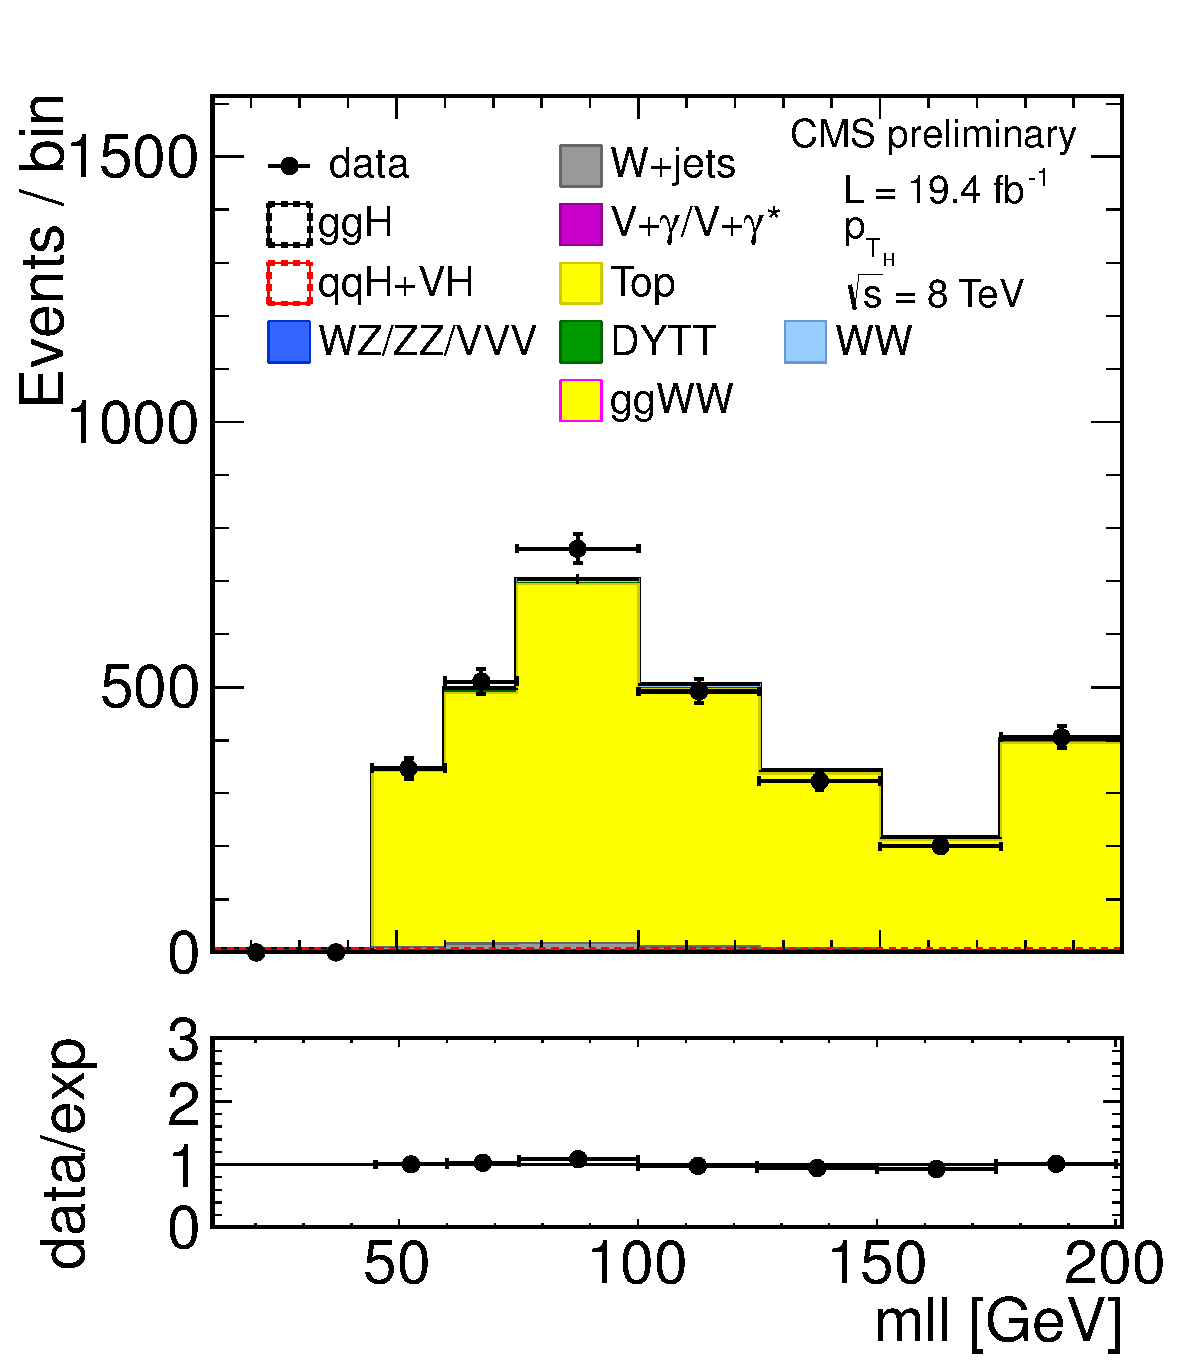
\includegraphics[width=0.35\textwidth]{images/mllBin1CtrlDD.pdf}}

\subfigure[$45\GeV<\pth<85\GeV$]{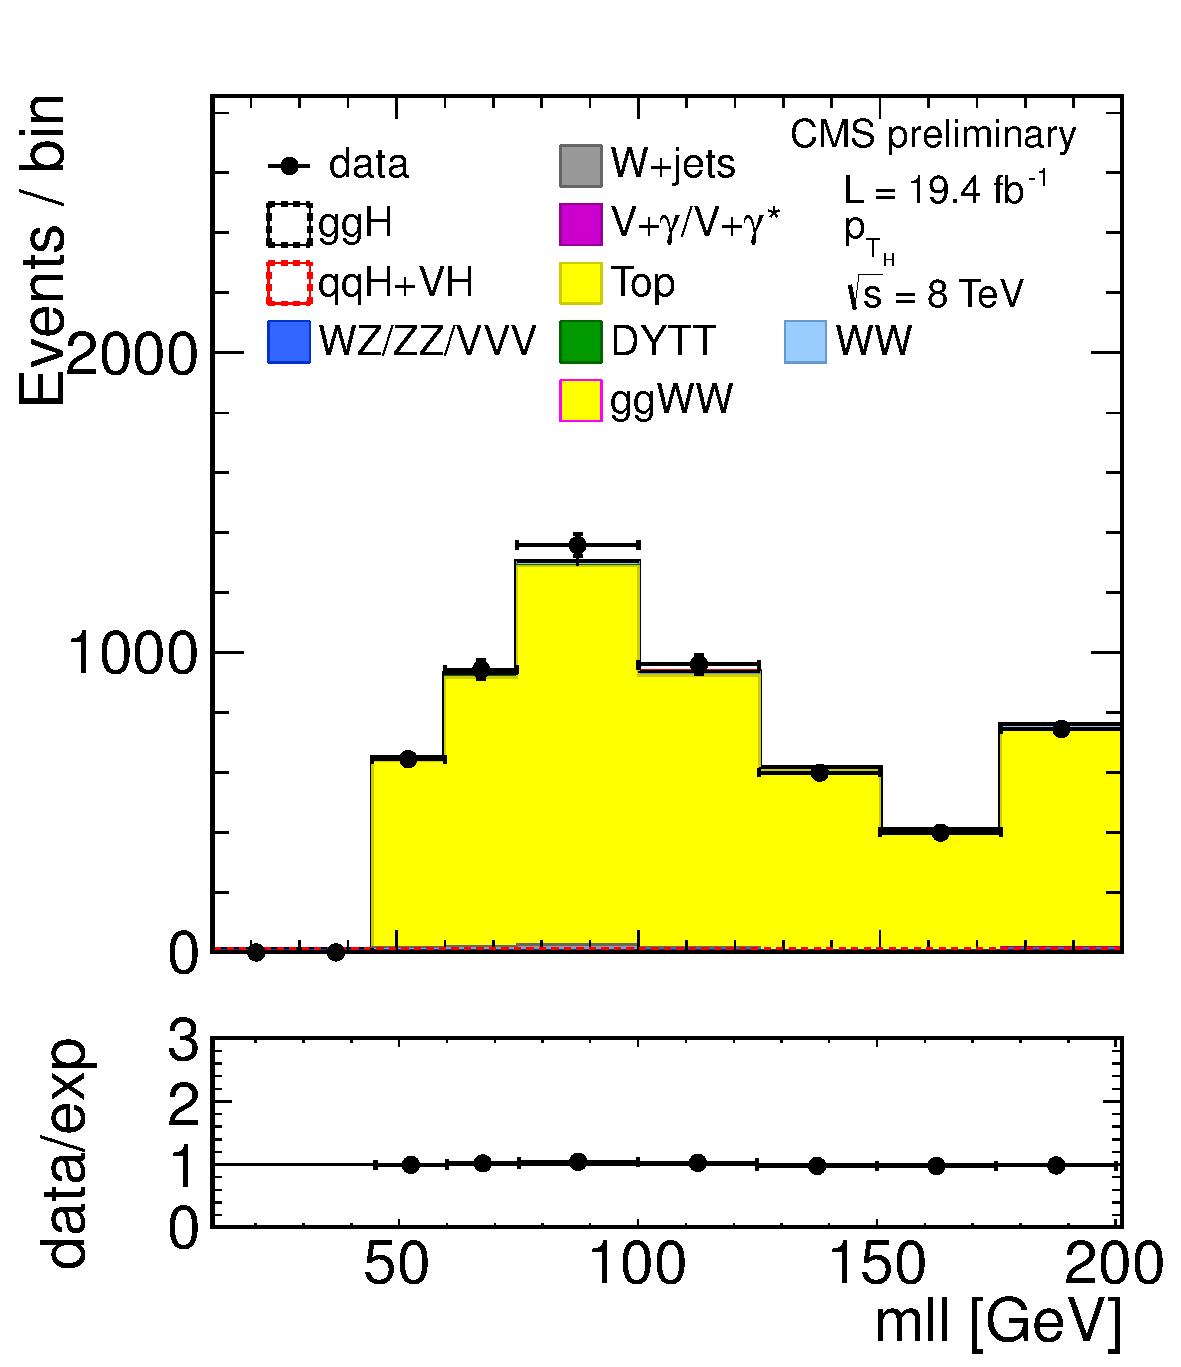
\includegraphics[width=0.35\textwidth]{images/mllBin2CtrlDD.pdf}}
\subfigure[$85\GeV<\pth<125\GeV$]{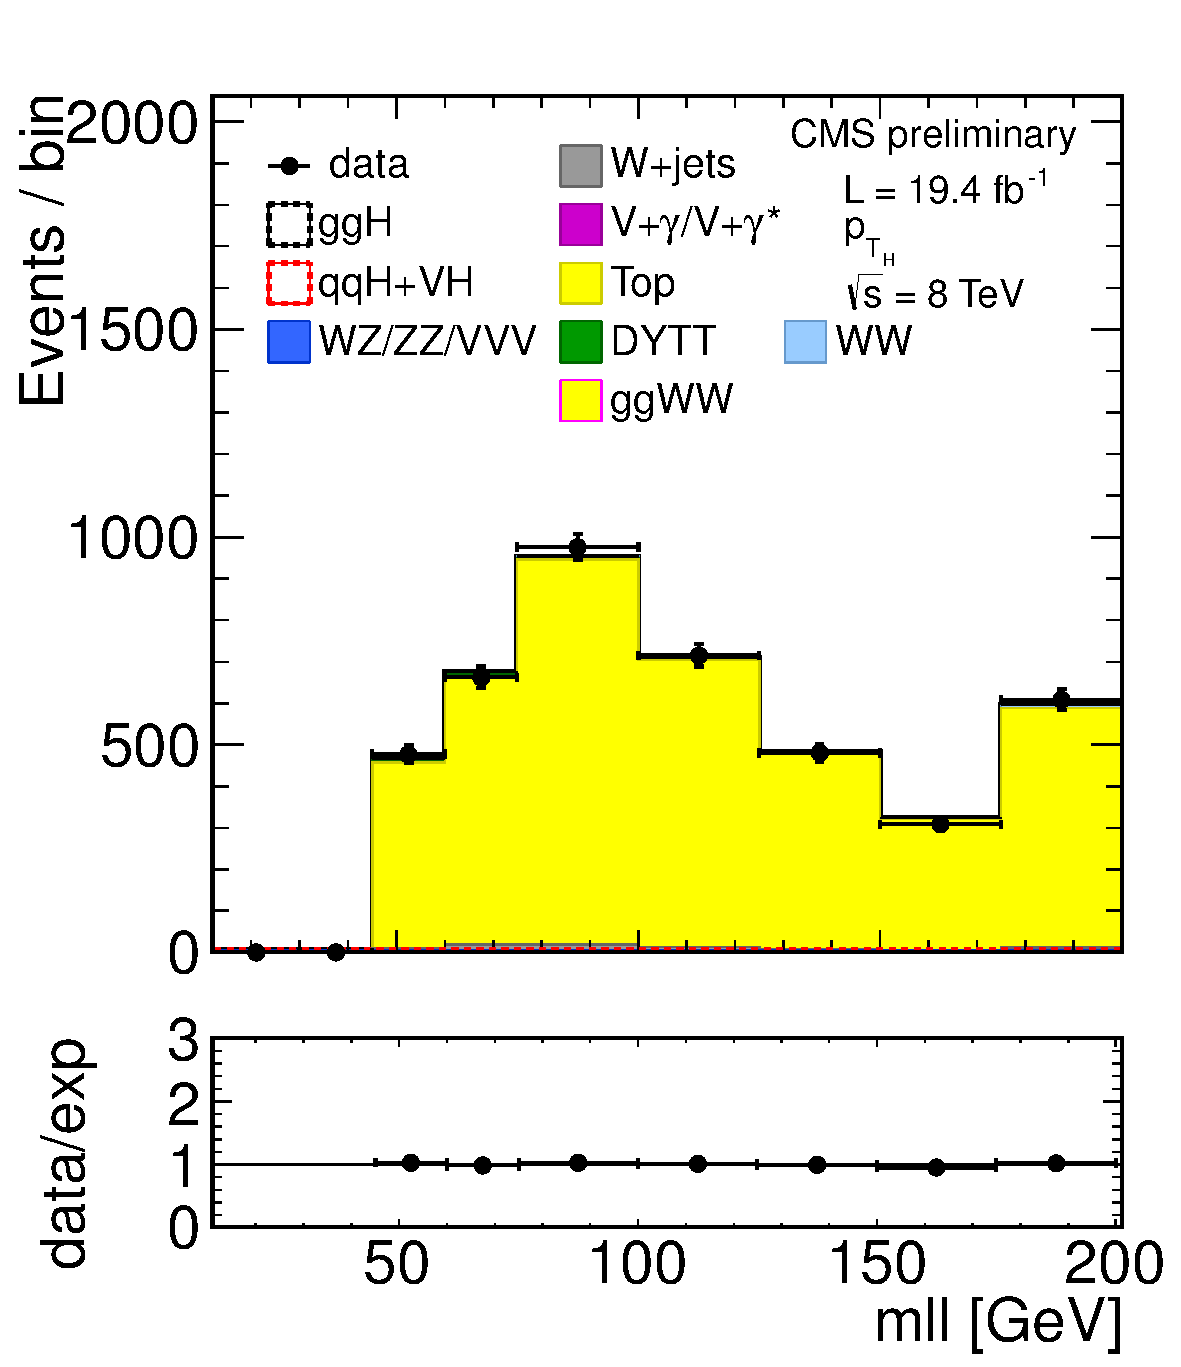
\includegraphics[width=0.35\textwidth]{images/mllBin3CtrlDD.pdf}}

\subfigure[$125\GeV<\pth<165\GeV$]{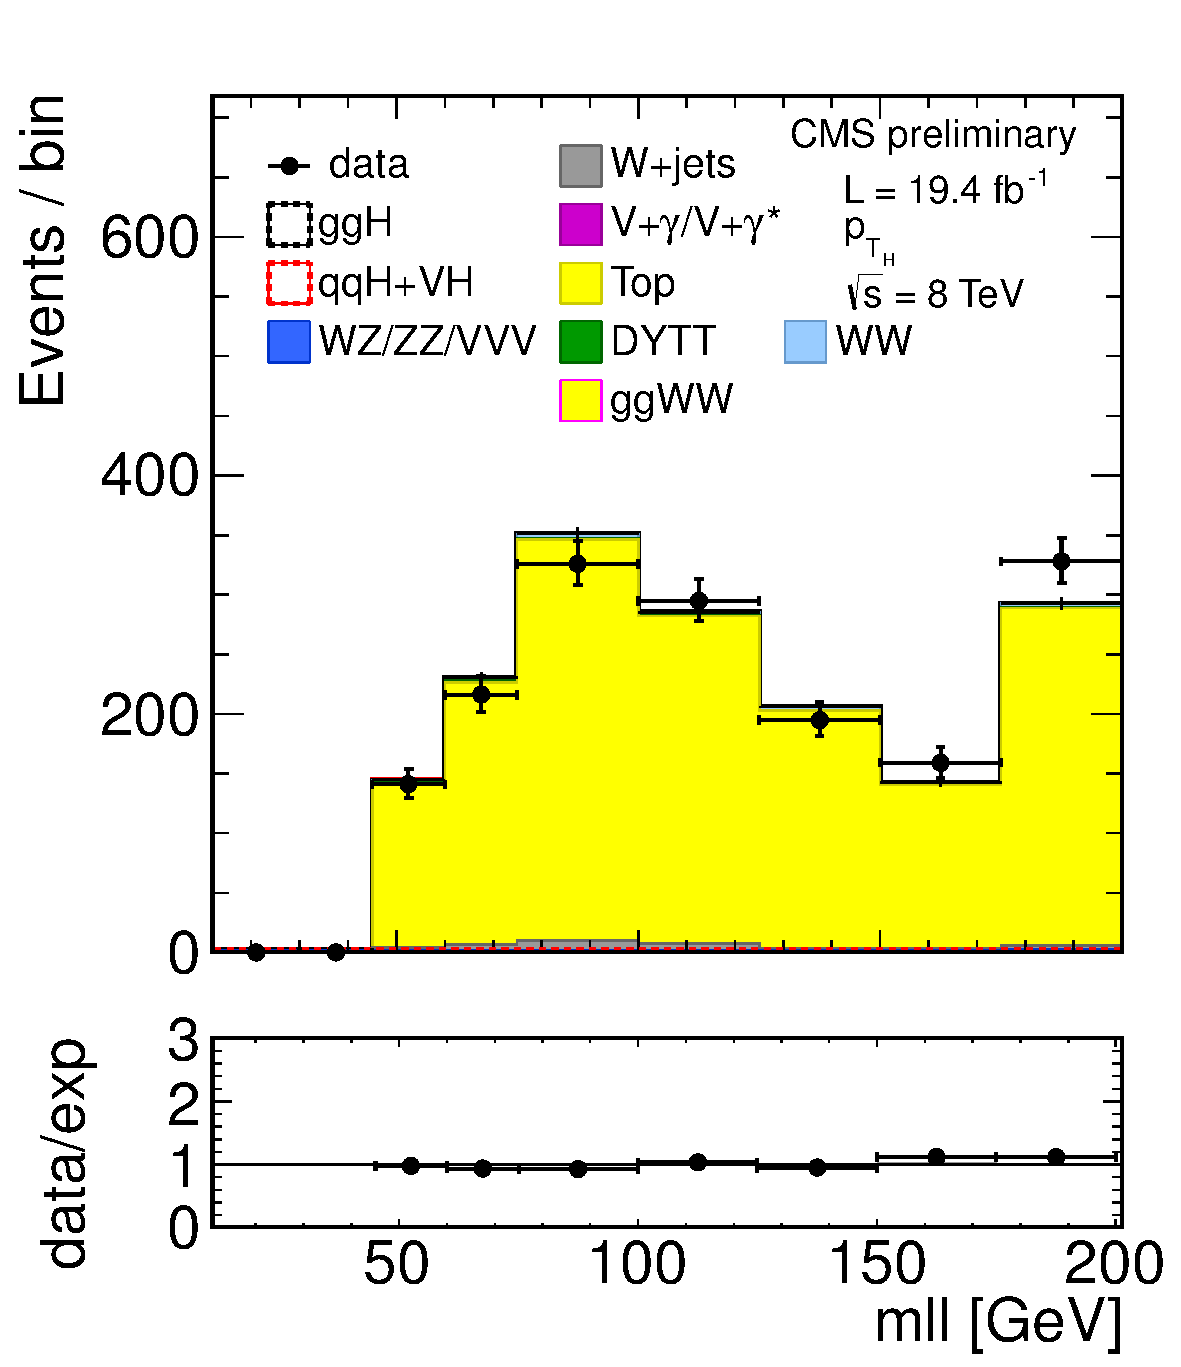
\includegraphics[width=0.35\textwidth]{images/mllBin4CtrlDD.pdf}}
\subfigure[$\pth>165\GeV$]{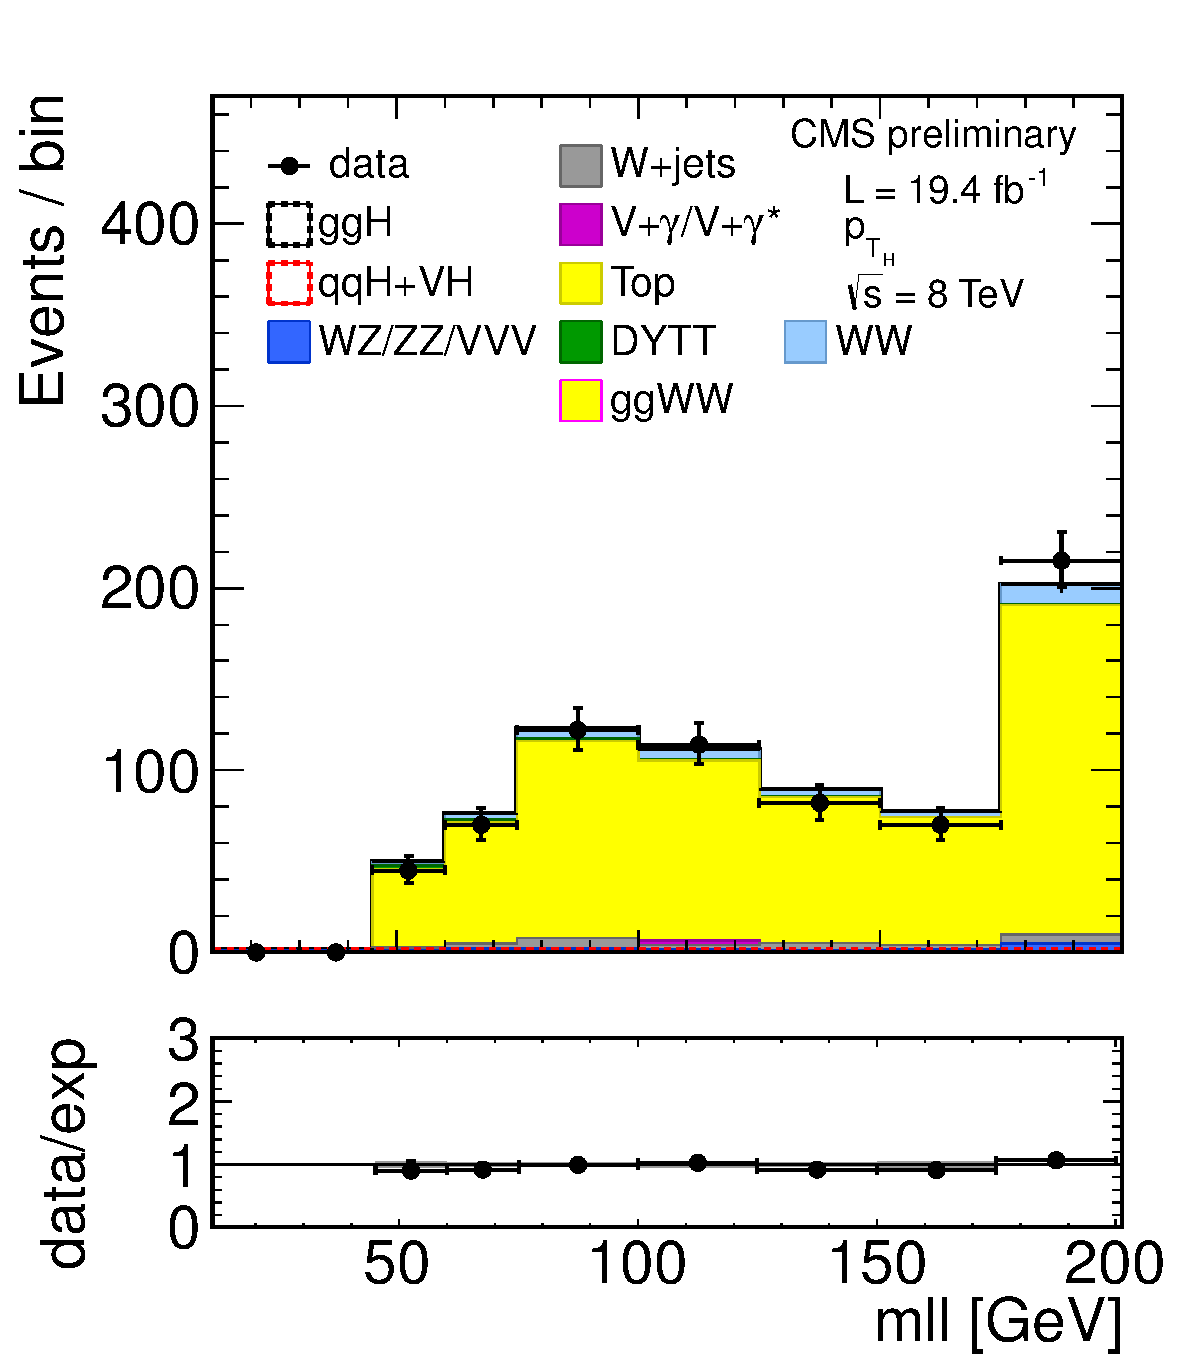
\includegraphics[width=0.35\textwidth]{images/mllBin5CtrlDD.pdf}}
\caption{$\mll$ distributions in the CtrlDD region for the different $\pth$ bins.\label{fig:mllCtrlDD}}
\end{figure}

























\clearpage
\subsection{WW background \label{sec:WWBackground}}

For what the $\mathrm{qq\to W^{+}W^{-}}$ background shape is concerned, the prediction from the simulation is used.
This background is divided into six different parts, corresponding to the six \pth bins defined in the analysis. The normalization of the $\mathrm{qq\to W^{+}W^{-}}$ background is left free to float in each bin, in such a way to adjust it in order to match the data during the fit procedure. In this way the shape difference between the $p_\mathrm{T}^\mathrm{WW}$ theory prediction and the distribution provided by the simulation, which is obtained with the \textsc{Madgraph} generator, is minimized.\\
In figure \ref{fig:ww_wwnlo} a comparison is shown between the $p_\mathrm{T}^\mathrm{WW}$ spectra of two different $\mathrm{qq\to W^{+}W^{-}}$ samples: one obtained with the \textsc{Madgraph} generator and the other after applying to the same distribution a reweighting in order to match the theoretical prediction at NLO+NNLL precision.

\begin{figure}[b]
\centering
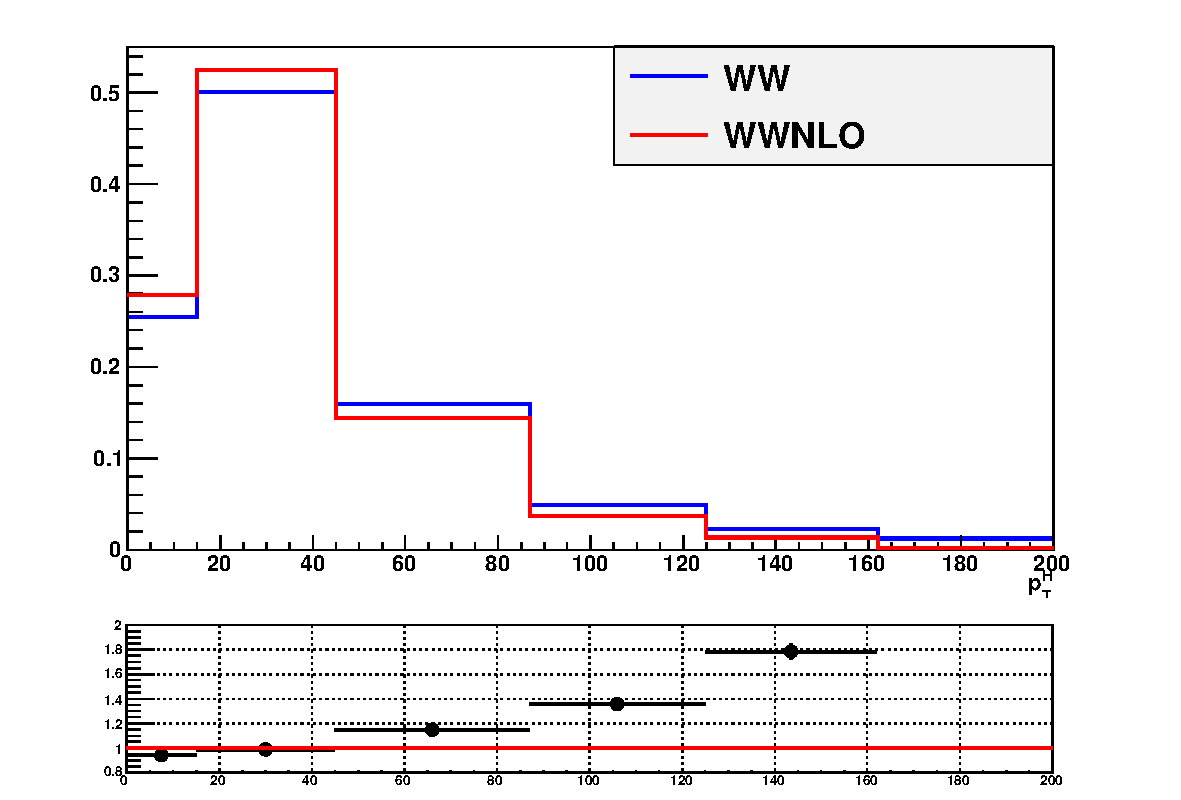
\includegraphics[width=0.7\textwidth]{images/WWnlo/WW_WWnlo.pdf}
\caption{Comparison between the $p_\mathrm{T}^\mathrm{WW}$ distributions obtained with two different MC generators: the blue line corresponds to the \textsc{Madgraph} generator and the red line refers to he same sample in which a reweighting has been applied in order to match the theoretical prediction at NLO+NNLL precision. }\label{fig:ww_wwnlo}
\end{figure}

A shape discrepancy can be clearly observed and the effect becomes larger at high values of \pth.
In order to assess the effect of this discrepancy on the shapes of the variables used for the signal extraction, \mll and \mt, the shapes have been checked in all \pth bins, comparing different MC samples. The \textsc{Madgraph} sample used for the nominal shape is compared to the \textsc{Madgraph} sample with NLO+NNLL  reweighting, a \textsc{Powheg} sample with NLO accuracy and an \textsc{aMC@NLO} sample.
The results of this comparison are shown in figures \ref{fig:ww_mll} and \ref{fig:ww_mth}. The shape discrepancy among the different models is included as an additional systematic uncertainty.

\begin{figure}[htb]
\centering
\subfigure[$0<\pth<15$\GeV]{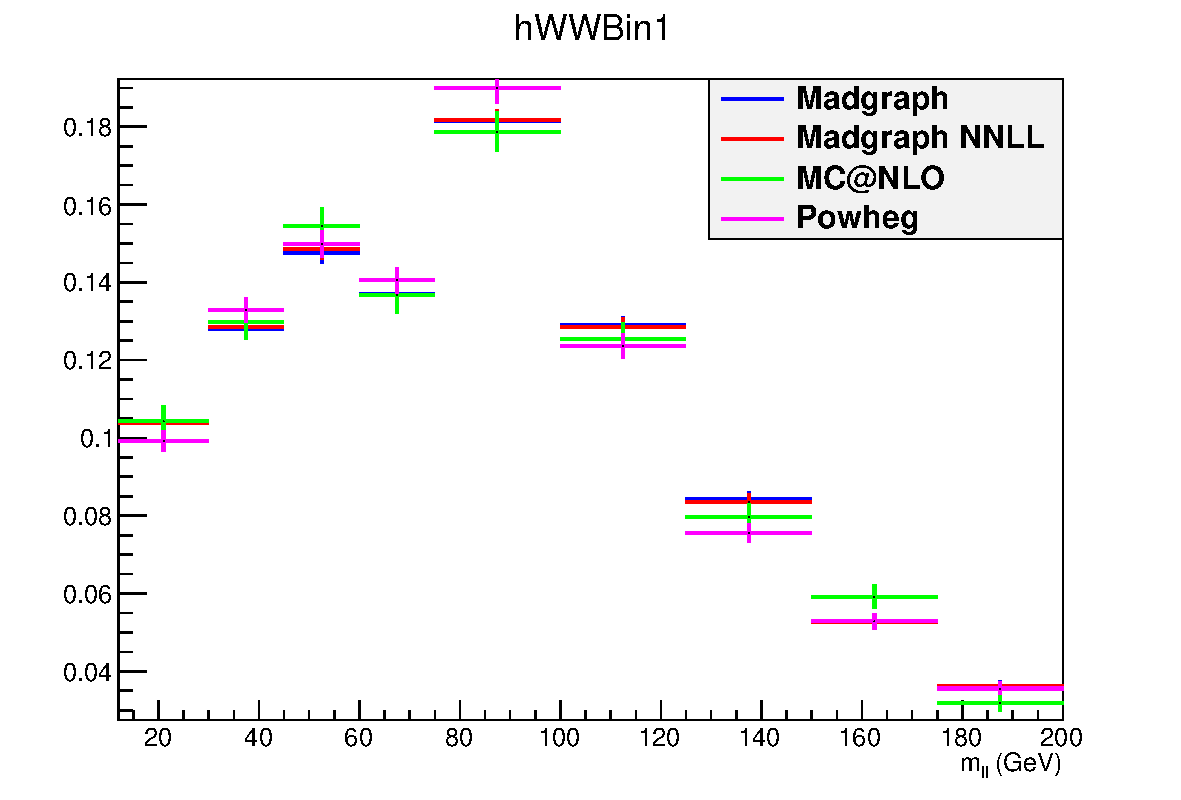
\includegraphics[width=0.4\textwidth]{images/WWnlo/mllBin1.pdf}}
\subfigure[$15<\pth<45$\GeV]{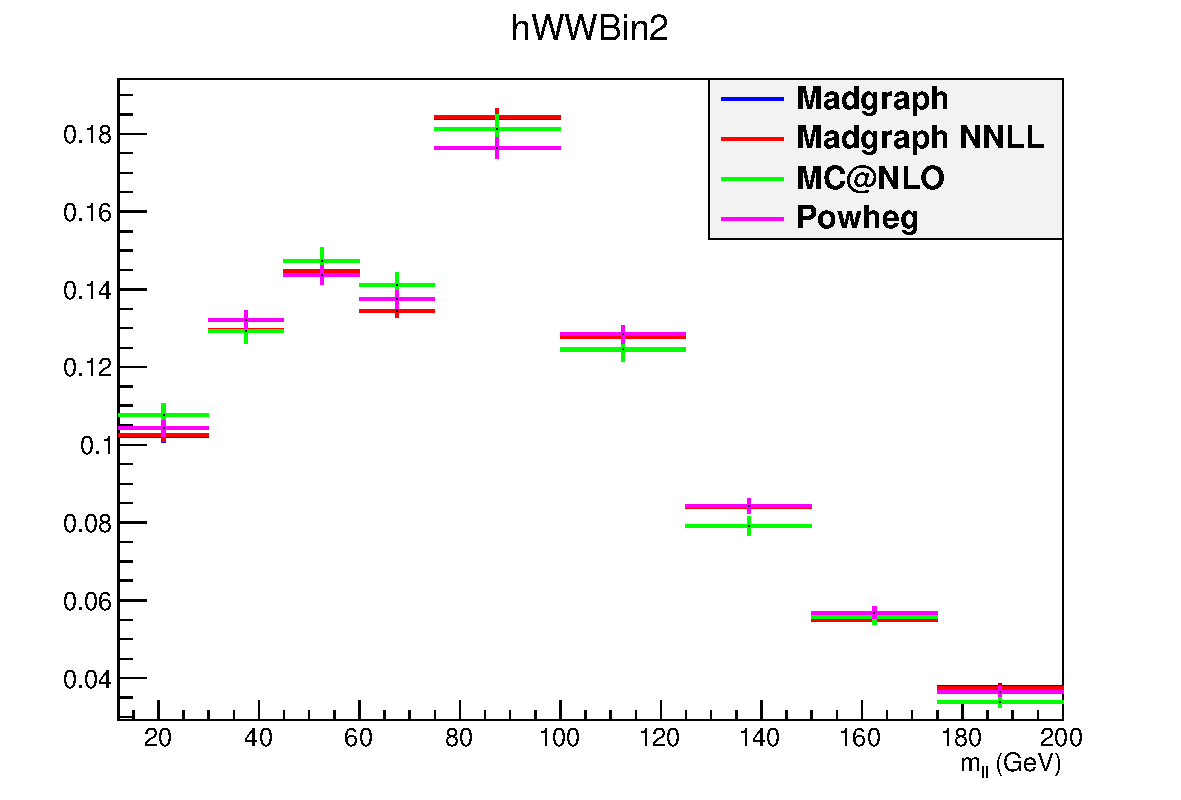
\includegraphics[width=0.4\textwidth]{images/WWnlo/mllBin2.pdf}}\\
\subfigure[$45<\pth<85$\GeV]{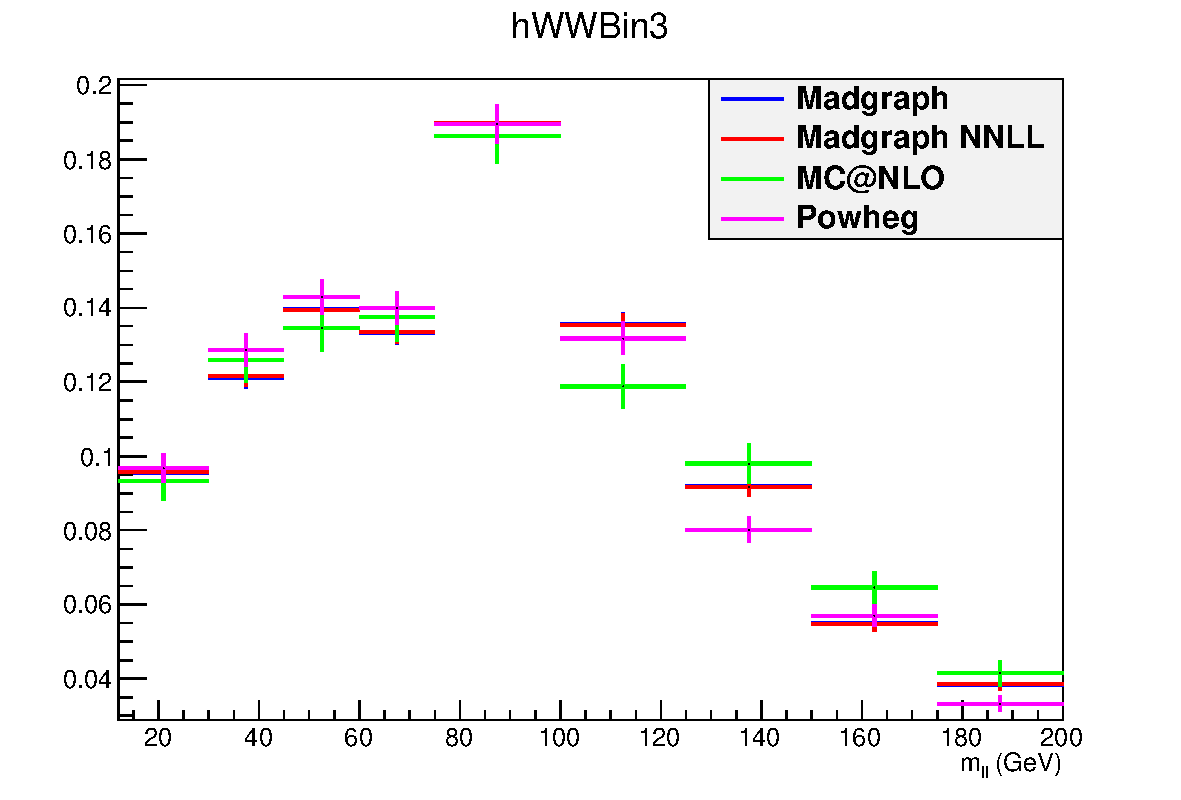
\includegraphics[width=0.4\textwidth]{images/WWnlo/mllBin3.pdf}}
\subfigure[$85<\pth<125$\GeV]{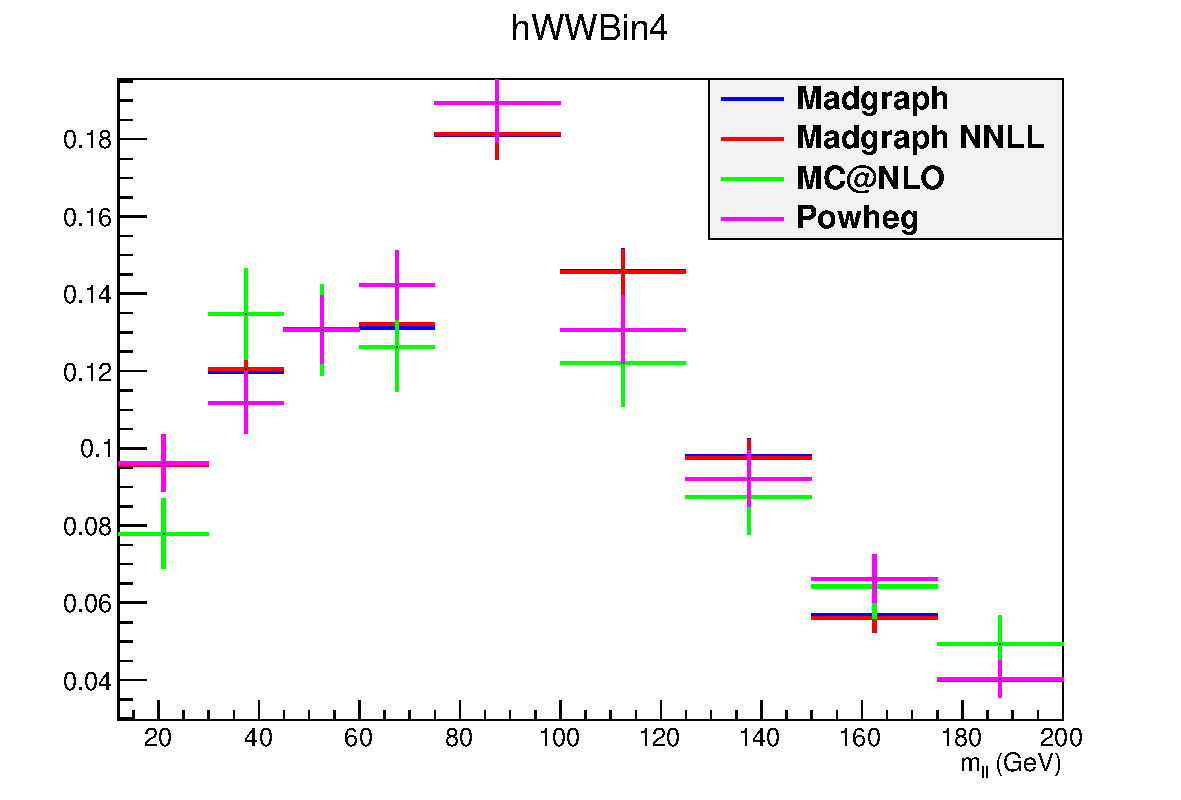
\includegraphics[width=0.4\textwidth]{images/WWnlo/mllBin4.pdf}}\\
\subfigure[$125<\pth<165$\GeV]{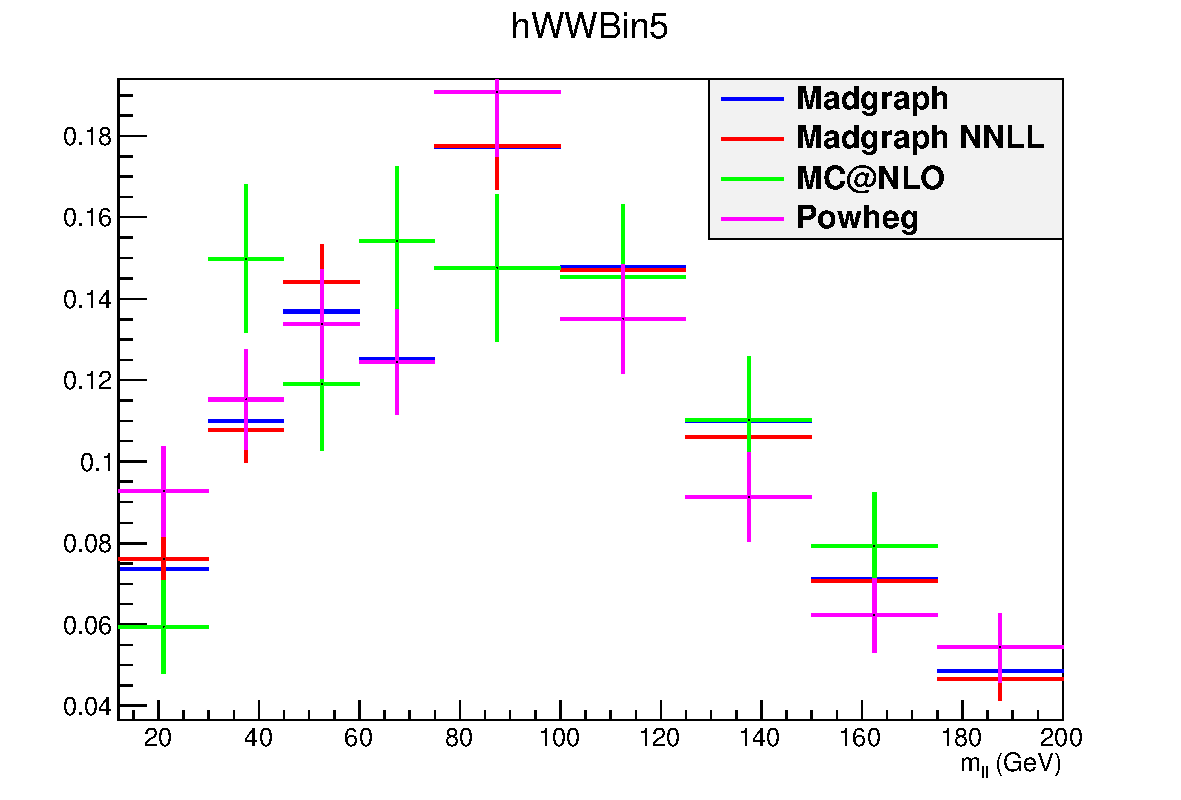
\includegraphics[width=0.4\textwidth]{images/WWnlo/mllBin5.pdf}}
\subfigure[$\pth>165$\GeV]{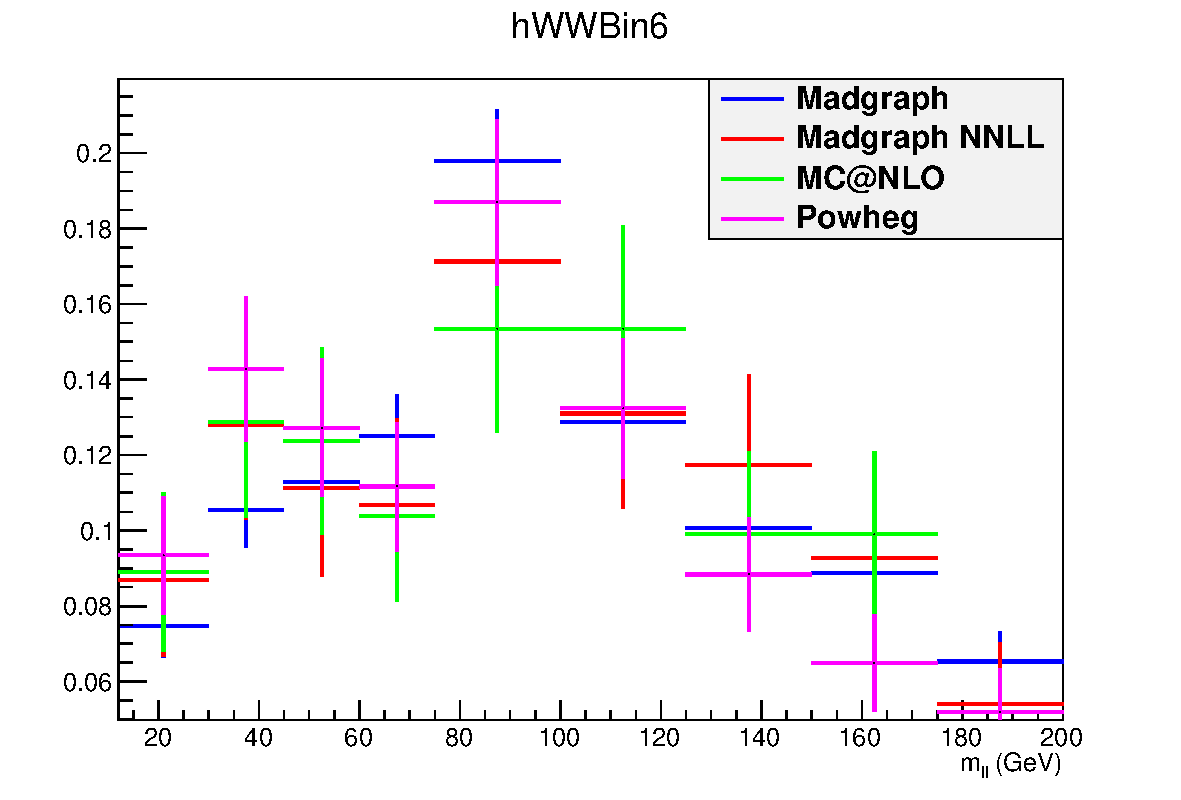
\includegraphics[width=0.4\textwidth]{images/WWnlo/mllBin6.pdf}}\\
\caption{Comparison between the default WW background sample and other theoretical models for the \mll distributions in every \pth bin.\label{fig:ww_mll}}
\end{figure}

\begin{figure}[htb]
\centering
\subfigure[$0<\pth<15$\GeV]{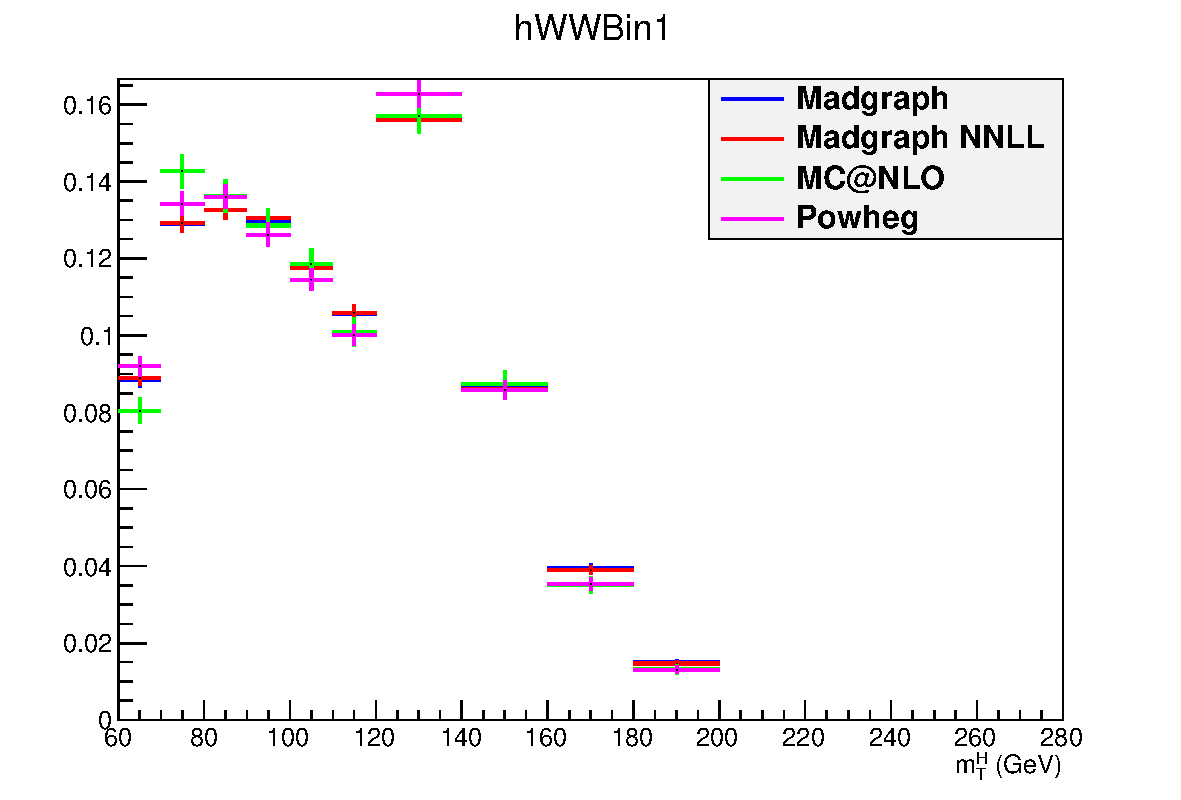
\includegraphics[width=0.4\textwidth]{images/WWnlo/mthBin1.pdf}}
\subfigure[$15<\pth<45$\GeV]{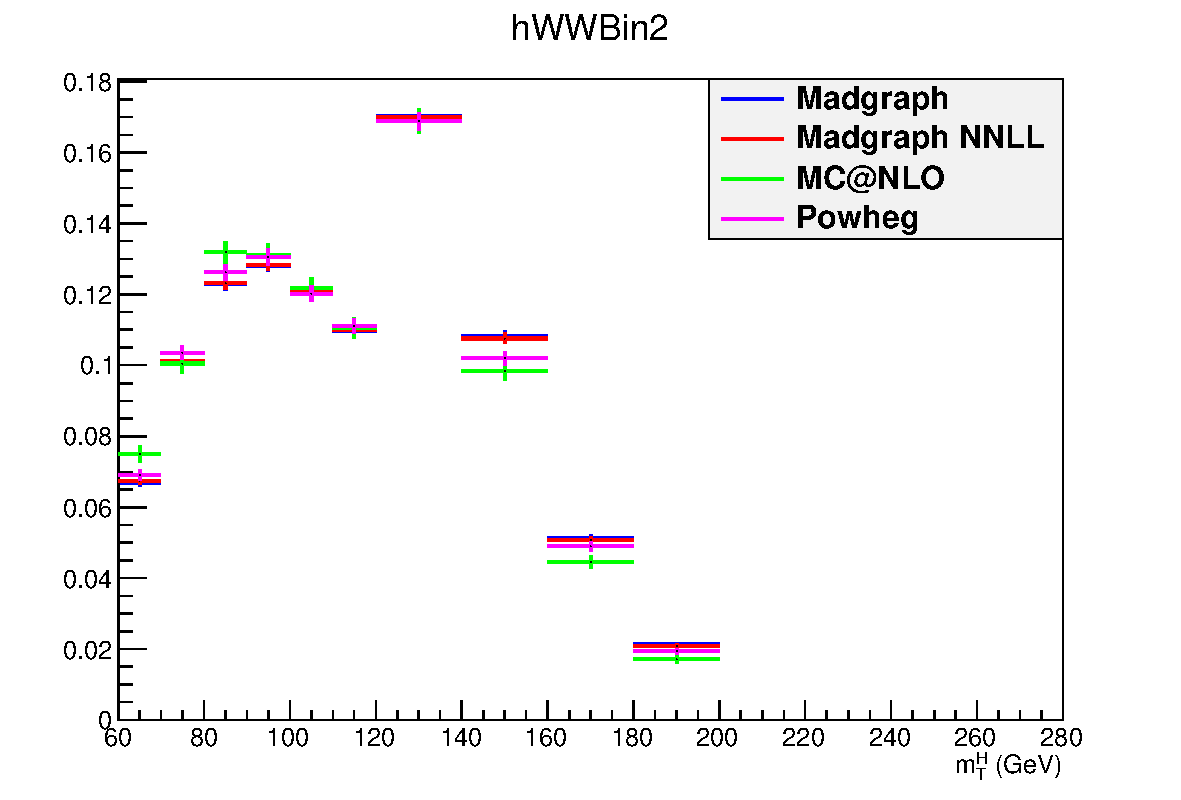
\includegraphics[width=0.4\textwidth]{images/WWnlo/mthBin2.pdf}}\\
\subfigure[$45<\pth<85$\GeV]{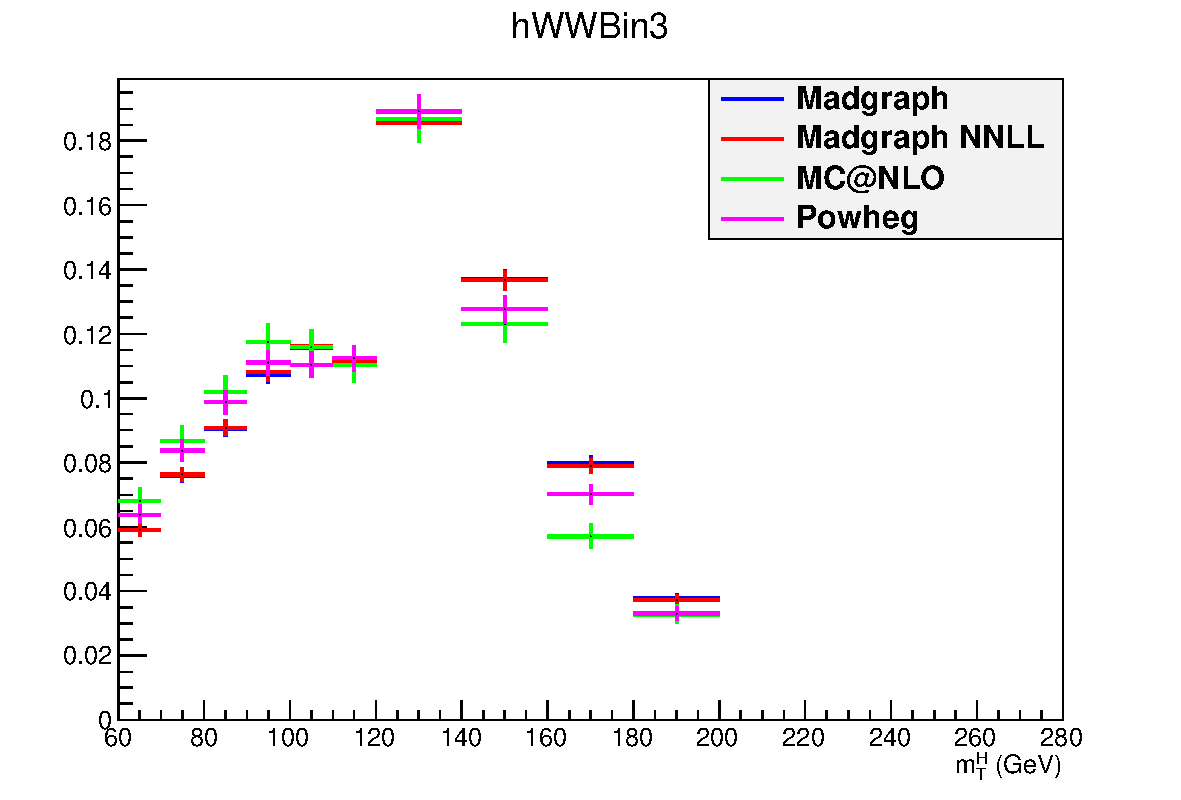
\includegraphics[width=0.4\textwidth]{images/WWnlo/mthBin3.pdf}}
\subfigure[$85<\pth<125$\GeV]{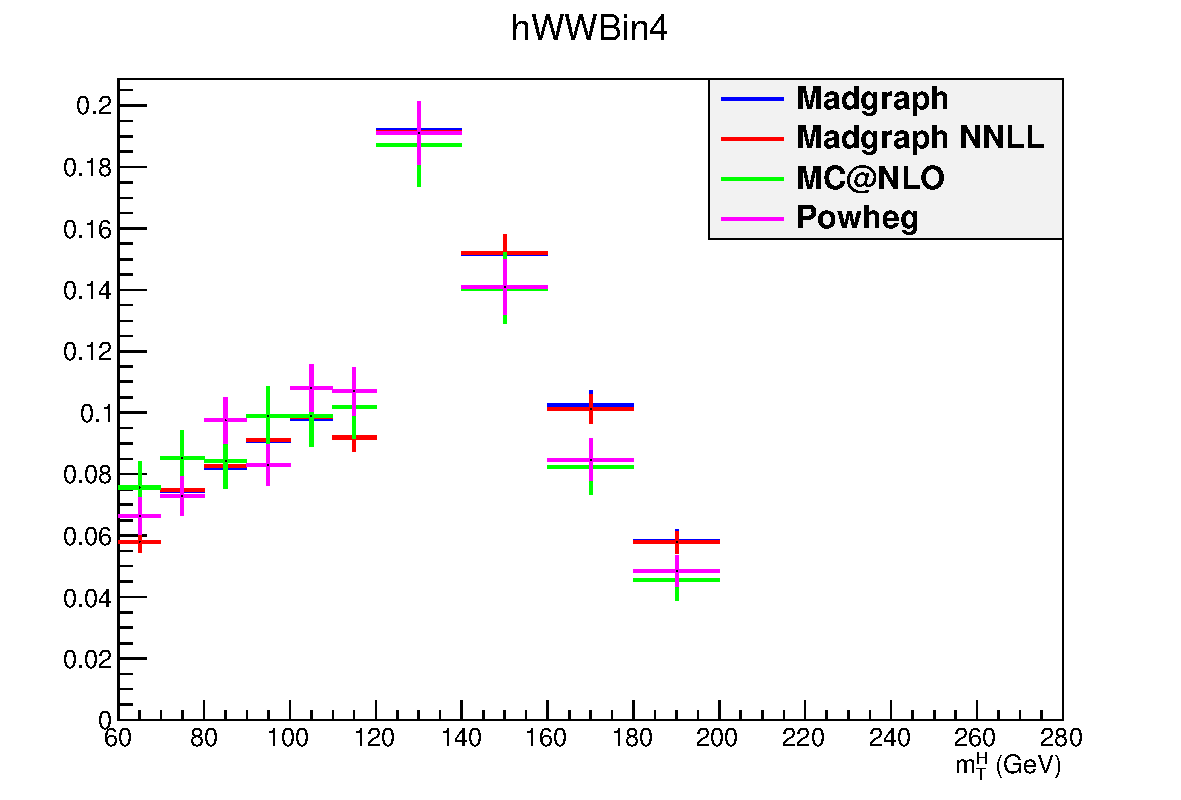
\includegraphics[width=0.4\textwidth]{images/WWnlo/mthBin4.pdf}}\\
\subfigure[$125<\pth<165$\GeV]{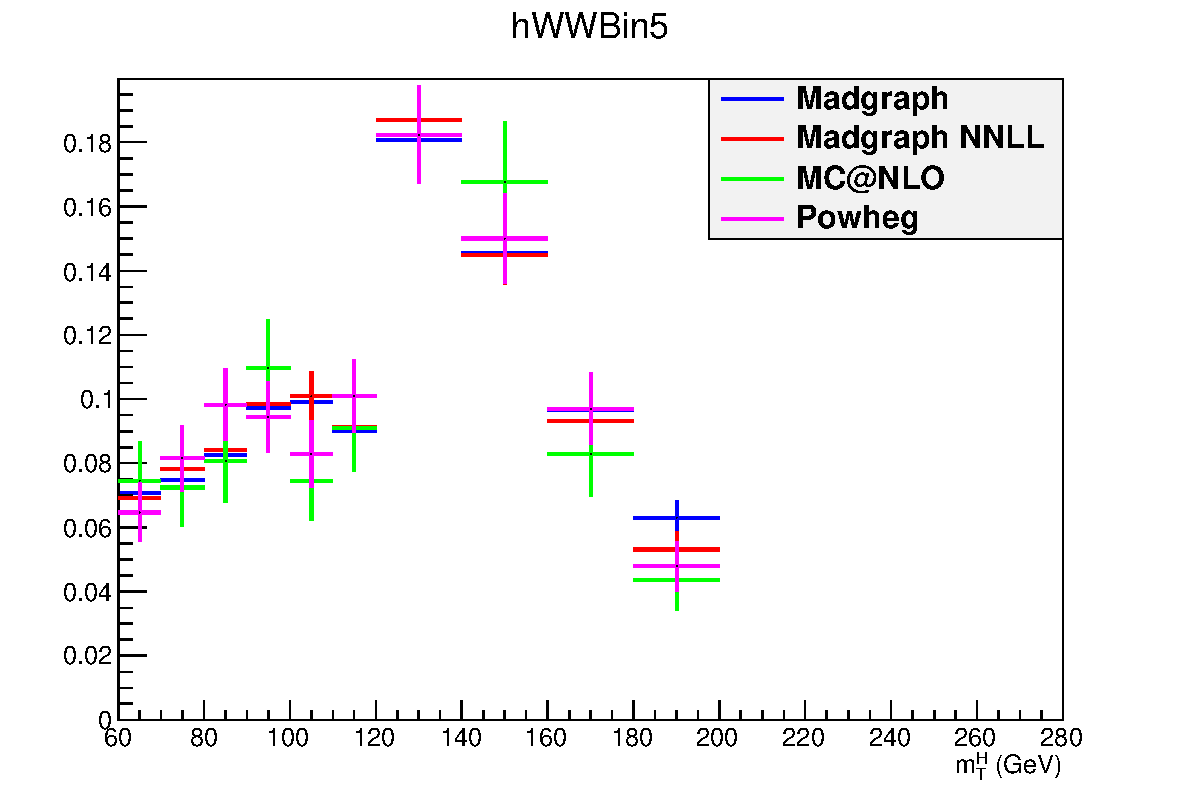
\includegraphics[width=0.4\textwidth]{images/WWnlo/mthBin5.pdf}}
\subfigure[$\pth>165$\GeV]{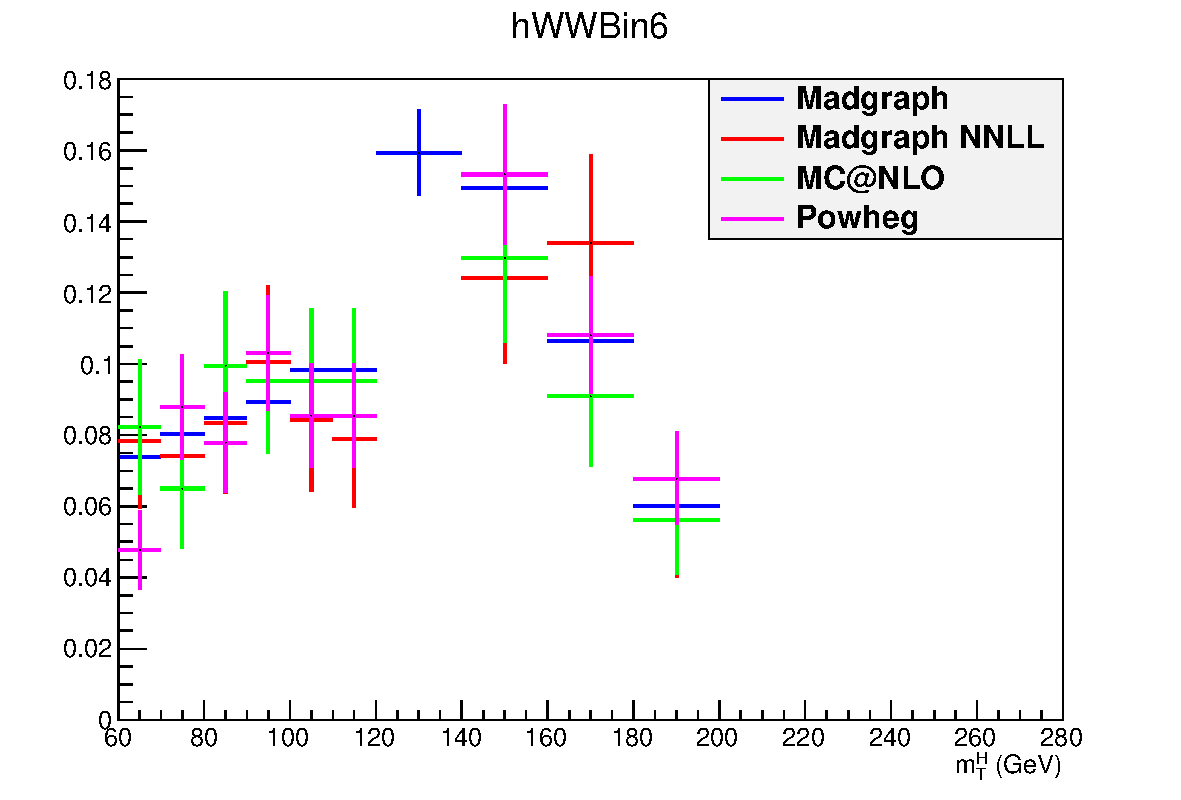
\includegraphics[width=0.4\textwidth]{images/WWnlo/mthBin6.pdf}}\\
\caption{Comparison between the default WW background sample and other theoretical models for the \mt distributions in every \pth bin.\label{fig:ww_mth}}
\end{figure}

The gluon-induced WW process, i.e. gg$\to \mathrm{W^{+}W^{-}}$, has a sub-dominant contribution with respect to the quark-induced process, being the cross section ratio between the two of about 5\%. The \mll and \mt shapes for this background are taken from simulation while the cross section is scaled to the approximate NLO calculation~\cite{Bonvini:2013jha,Passarino:2013bha}.

The agreement of the \mll and \mt shapes between simulation and data for this background was checked in a signal-free control, defined selecting events with values of \mll greater than 70\GeV. A comparison of the \mll and \mt shapes in data and simulation is shown in Fig.~\ref{fig:WW} for events containing zero and one jets, inclusive in \pth.

\begin{figure}[htb]
\centering
\subfigure[\mll{} -- 0 jets]{
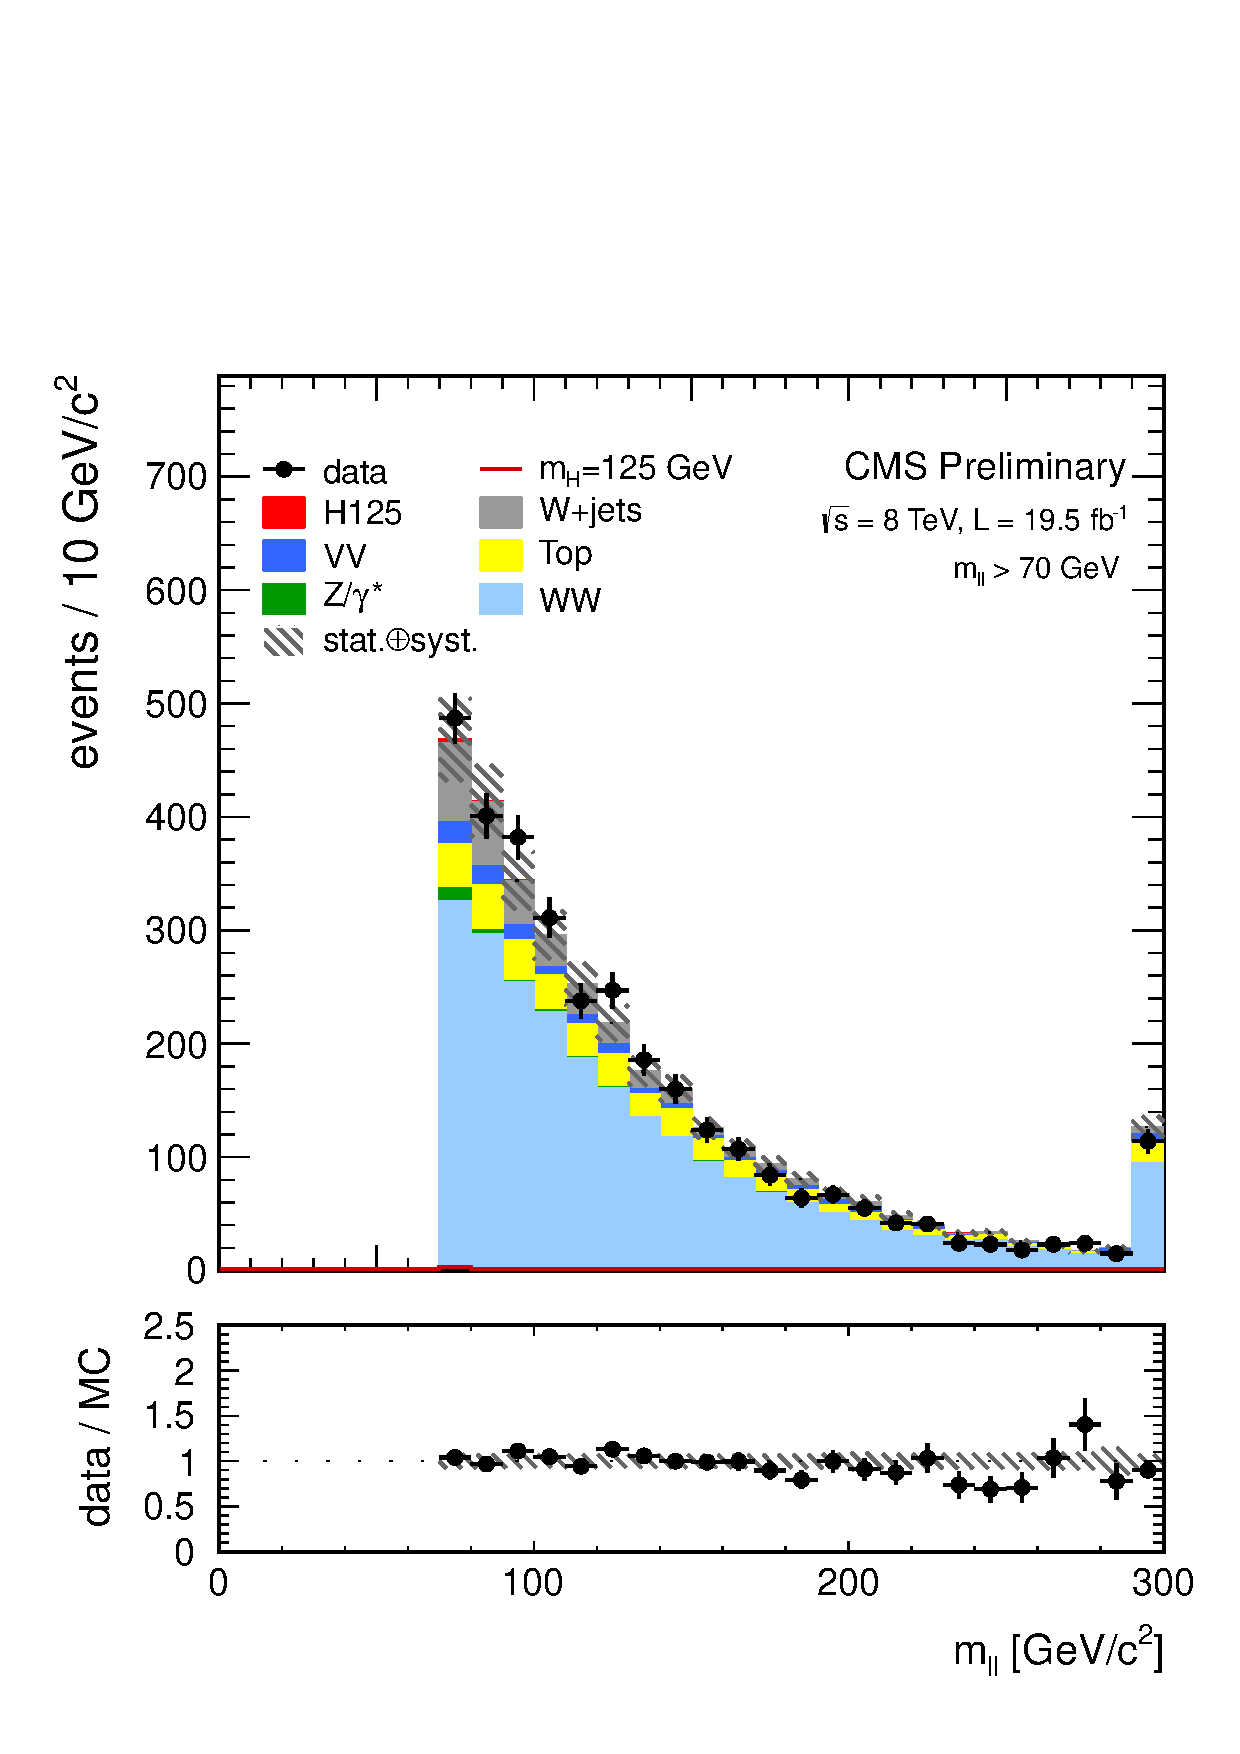
\includegraphics[width=0.4\textwidth]{images/WWctrl/mll0j.pdf}
}
\subfigure[\mt{} -- 0 jets]{
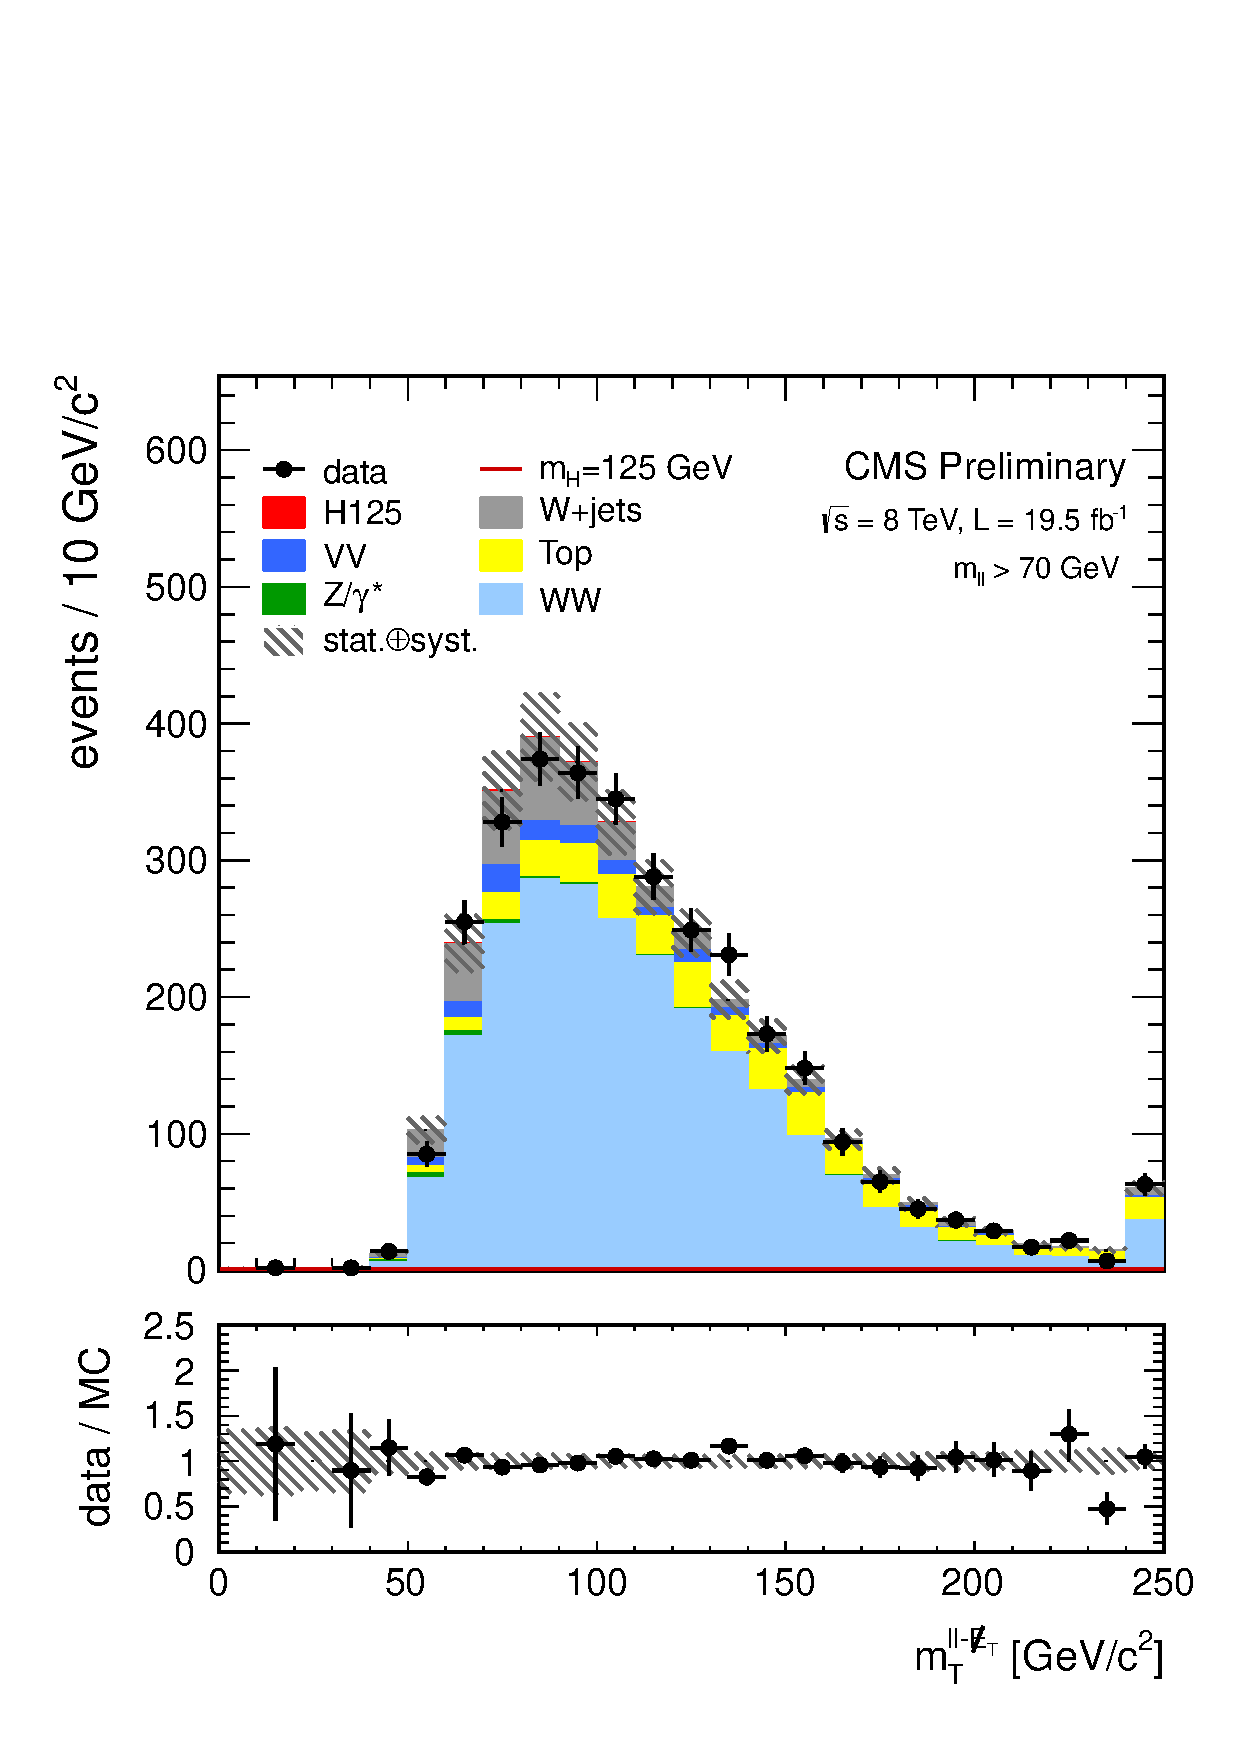
\includegraphics[width=0.4\textwidth]{images/WWctrl/mt0j.pdf}
}
\\
\subfigure[\mll{} -- 1 jet]{
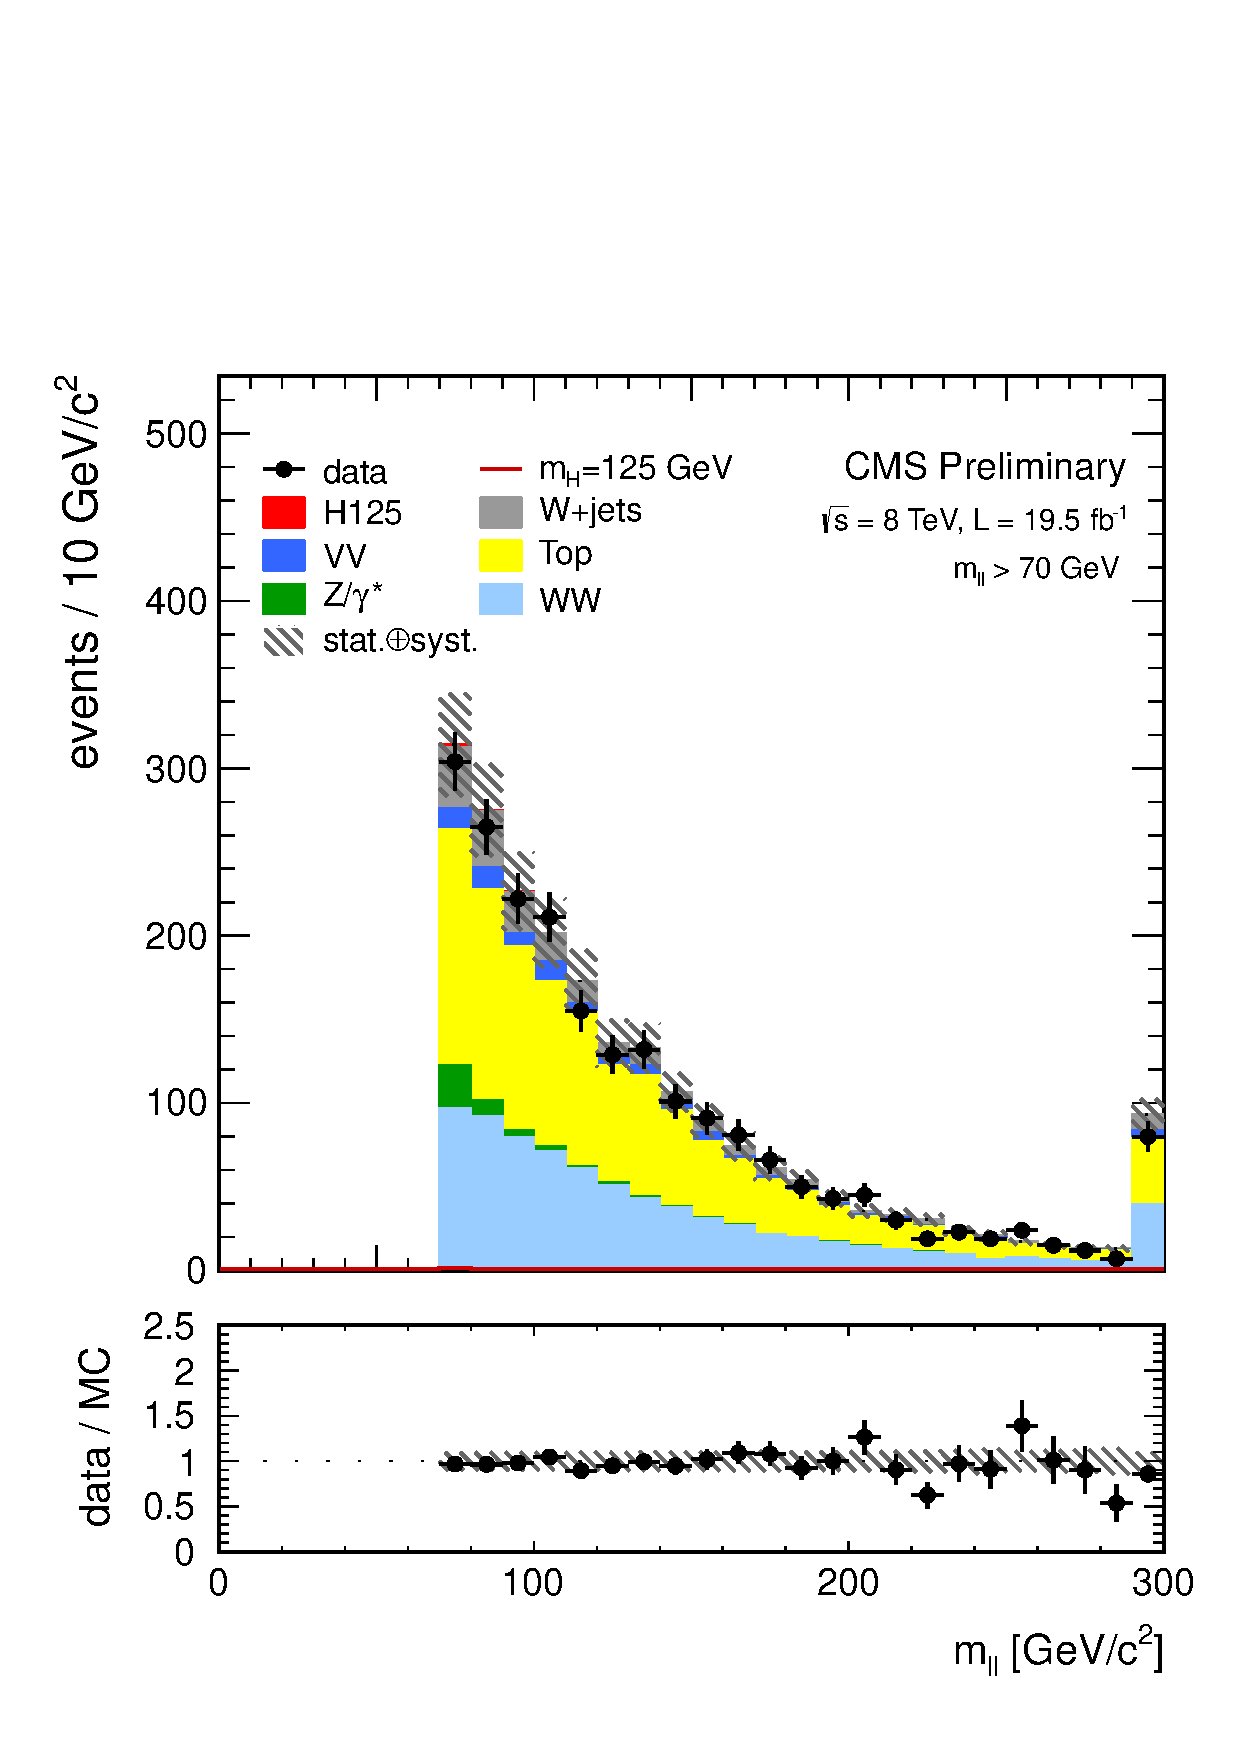
\includegraphics[width=0.4\textwidth]{images/WWctrl/mll1j.pdf}
}
\subfigure[\mt{} -- 1 jet]{
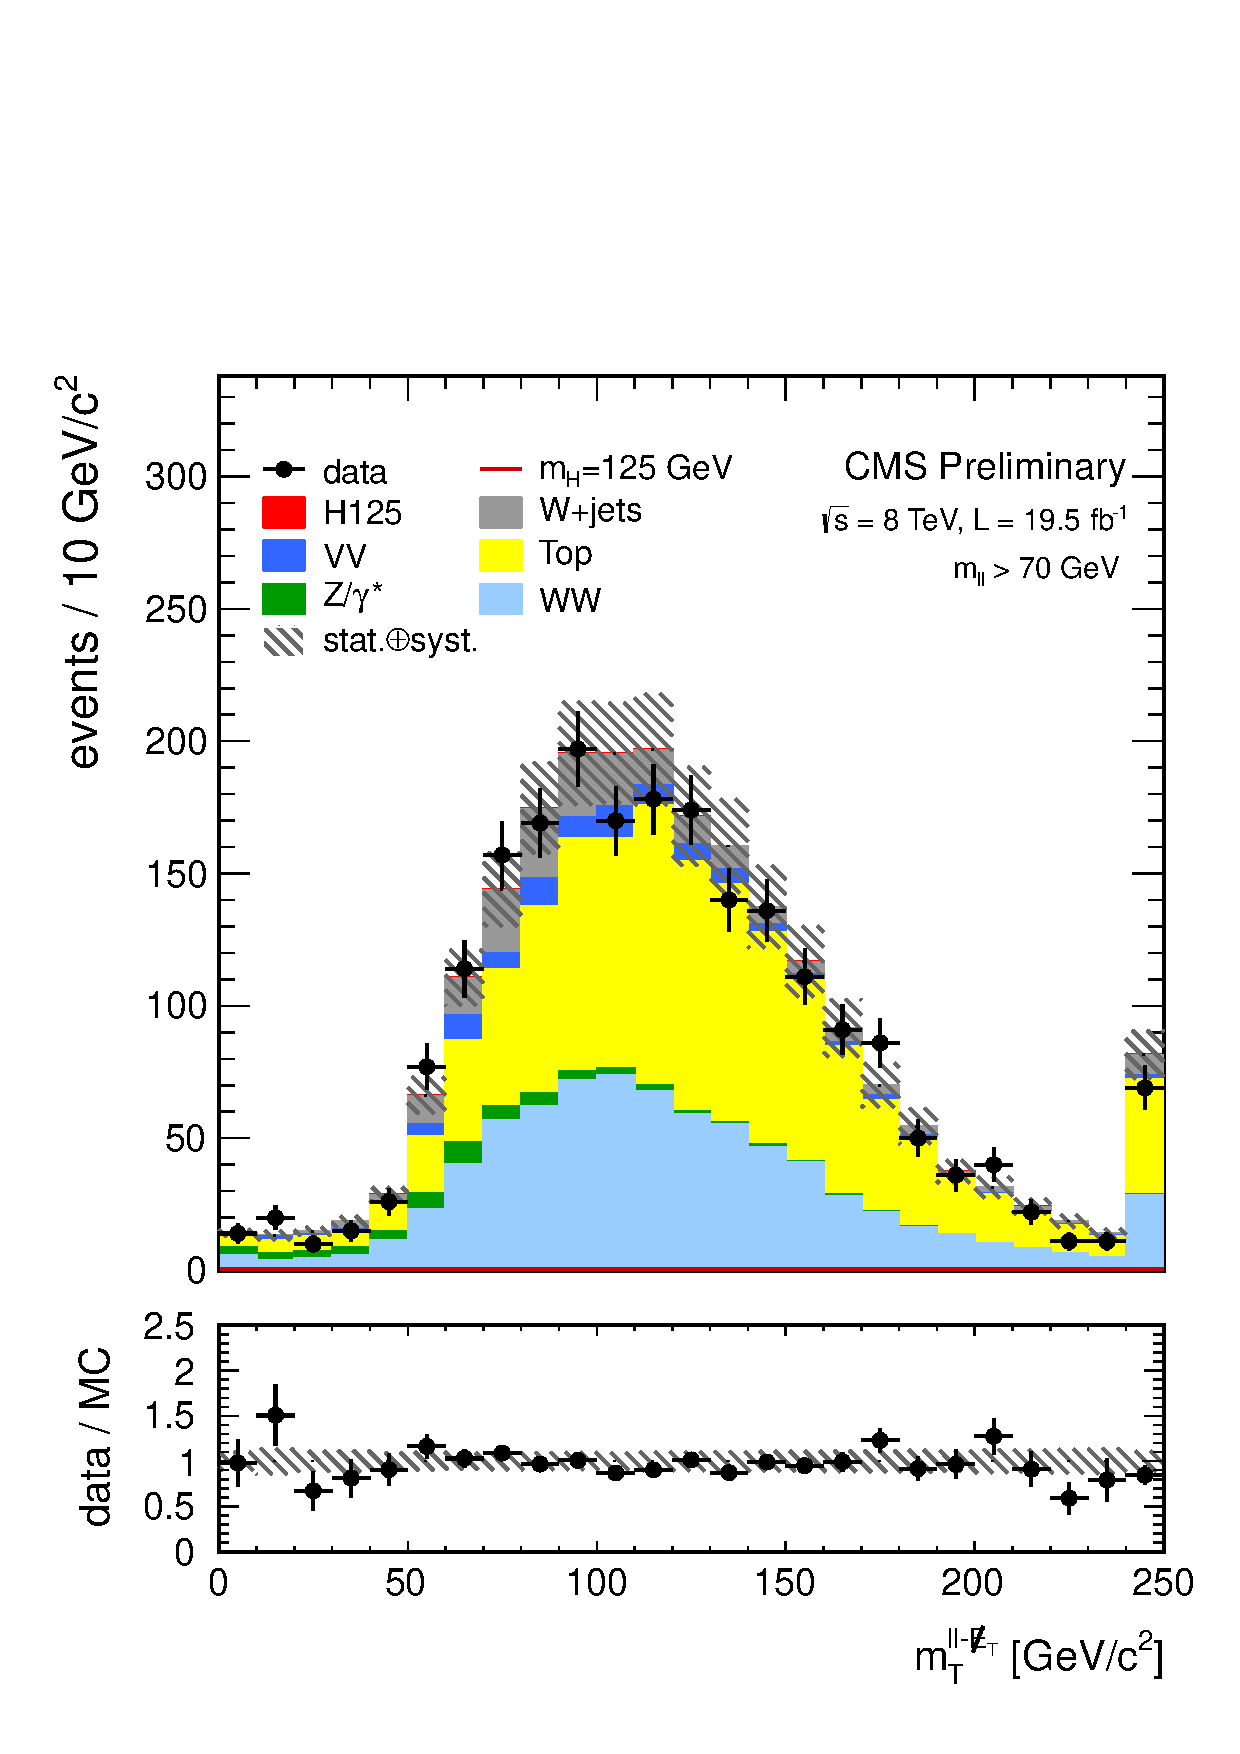
\includegraphics[width=0.4\textwidth]{images/WWctrl/mt1j.pdf}
}

\caption{Comparison of the \mll and \mt shapes in data and simulation for events with zero and 1 jets, inclusive in \pth. The events are required to pass the analysis requirements and, in order to define a signal-free control region, to have $\mll > 70$\GeV.\label{fig:WW}}
\end{figure}











































\subsection{Other backgrounds\label{sec:OtherBackgrounds}}

	%------------------------------------------------------------------------------------
	\subsubsection{W+jets background\label{sec:wjetsbkg}}	
	
Events in which W bosons are produced in association with jets, as well as multi-jet events, constitute a background for this analysis, because one or more jets can be misidentified as leptons. The rate at which jets are misidentified as leptons may be not accurately described in simulation, hence a data driven method is used to estimate this background. 
	
The idea is to estimate the background containing one or two fake leptons selecting events with relaxed lepton quality criteria, i.e. looser with respect to the selections used at the analysis level, and computing the efficiencies for real and fake leptons to pass the tight lepton quality requirements of the analysis. 
A data-driven approach is pursued to estimate this background. A set of loosely selected lepton-like objects, referred to as the ``fakeable object' or ``denominator'' from here on, is defined in a data set of events dominated by dijet production.
To measure the fake rate we count how many fakeable objects pass the full lepton selection 
of the analysis, parameterized as a function of the phase space of the fakeable lepton, therefore 
it is extracted in bins of $\eta$ and \pt.
The ratio of the fully identified lepton, referred as ``numerator'', to the 
fakeable objects is taken as the probability for a fakeable object to fake a lepton:

\begin{equation} \label{eq:fake_rate}
{Fake\ Rate } = \frac{\# of \ fully \ reconstructed \ leptons}{\# of \ fakeable \ objects} 
\end{equation}

It is then used to extrapolate from the loose leptons sample to a sample of leptons satisfying the  
full selection.

The definition of the denominator is of large impact in the systematic uncertainties related to this method. For the 2012 data taking period a summary of the selections used for the numerator and the denominator of Eq.~\eqref{eq:fake_rate} is shown below for electrons and muons respectively.
For electrons the denominator is defined by the following requirements:

\begin{itemize}
\item $\sigma_\mathrm{i\eta i\eta} < 0.01 (0.03)$ for barrel (endcap);
\item $|\Delta\phi_\mathrm{in}| < 0.15 (0.10)$ for barrel (endcap);
\item $|\Delta\eta_\mathrm{in}| < 0.007 (0.009)$ for barrel (endcap);
\item $H/E < 0.12 (0.10)$ for barrel (endcap);
\item electron conversion rejection;
\item $|d_0| < 0.02$\,cm;
\item $\frac{\sum_\mathrm{trk}E_\mathrm{T}}{\pt^\mathrm{ele}} < 0.2$;
\item $\frac{\sum_\mathrm{ECAL}E_\mathrm{T}}{\pt^\mathrm{ele}} < 0.2$;
\item $\frac{\sum_\mathrm{HCAL}E_\mathrm{T}}{\pt^\mathrm{ele}} < 0.2$.
\end{itemize}

For muons the selection are loosened with respect to the tight analysis selection requiring that:

\begin{itemize}
\item $|d_0| < 0.02$\,cm;
\item MVA isolation output $> -0.6$.
\end{itemize}

%shown in Table~\ref{tab:fake_muons} and \ref{tab_fake_electrons} for muons and electrons respectively.

%\begin{table}
%\centering
%\begin{tabular}{c c c}
%\hline
%Selection & Numerator & Denominator \\
%\hline\hline
%Muon ID & Global Muon + Tracker Muon & Tracker Muon \\
%\pt     & $\pt>20$\GeV & $\pt>20$\GeV \\
%$\eta$  & $|\eta|<2.4$ & $|\eta|<2.4$ \\
%Isolation & $(\mathrm{trackIso+caloIso})/\pt < 0.15$ & $(\mathrm{trackIso+caloIso})/\pt < 1$ \\
%\# inner tracker hits & $\mathrm{\# hits} > 10$ & $\mathrm{\# hits} > 10$ \\
%\# pixel hits & $\mathrm{\# hits} > 0$ & $\mathrm{\# hits} > 0$ \\
%Global $\chi^2$ & $\chi^2/\mathrm{ndof} < 10$ & -- \\
%$d0$ & $d0 < 0.02$\,cm & $d0 < 0.02$\,cm \\
%$dz$ & $dz < 1$\,cm & $dz < 1$\,cm \\
%\# valid SA hits & $>0$ & -- \\
%\# muon stations & $>1$ & -- \\
%\hline
%\end{tabular}
%\caption{Numerator and denominator selections for muons.\label{tab:fake_muons}}
%\end{table}

The dijet enriched data set used for the fake rate measurement, which is selected using single lepton triggers with low \pt thresholds, it is not a pure sample containing just fake leptons, but may still contain prompt leptons coming from the W and Z boson decays. To reject muons from the W decay, the events are required to have $\MET<20$\GeV and a W transverse mass below 20\GeV as well. Muons from the Z decay are instead remove requiring $m_{\mu\mu}>20$\GeV and $m_{\mu\mu} \notin [76,106]$\GeV. For electrons the Z mass peak veto is enlarged to $m_\mathrm{ee} \notin [60,120]$\GeV. Finally both electrons and muons are required to be isolated from the leading jet in the event, i.e. $\Delta\phi(\ell,j)>1$. The residual prompt lepton contamination from EW processes such as W/Z+jets production, which can bias the fake rate measurement, is estimated using simulation and subtracted from both the numerator and denominator. The contamination from EW processes is different for the numerator and denominator and is particularly important for relatively high lepton \pt values.

In addition to the fake rate, also a prompt lepton rate is evaluated, defined as the probability of a prompt lepton passing the loose requirements to also pass the tight analysis selections.
The prompt rate is also measured in data, defining a control region enriched in $\mathrm{Z} \to \ell\ell$ events, selecting dilepton events with an invariant mass of the two leptons in the Z peak mass region.

Both the fake and prompt rate are used to reweight the data samples used in the analysis in order to obtain directly from data the contribution of the fake lepton background. The method to apply those rates is explained below in the simple case of just one lepton in the data sample, i.e. data selected by single lepton triggers, but can be straightforwardly generalized to situations with more than one lepton.
Suppose that the total number of leptons passing the loose requirements, $N_\ell$, is made up of $N_p$ prompt and $N_f$ fake leptons. $N_p$ and $N_f$ cannot be directly measured but one can measure the number of events where no leptons, $N_{t0}$, or one lepton, $N_{t1}$, pass the tight analysis requirement. These numbers are related by the following equations:

\begin{equation}\label{eq:fake_single_lep}
\begin{gathered}
    N_\ell = N_p + N_f = N_{t0} + N_{t1}\\
    N_{t0} = (1-p)N_p + (1-f)N_f\\
    N_{t1} = pN_p + fN_f
\end{gathered}
\end{equation}

where $p$ and $f$ are the prompt and fake rates respectively. Equation~\eqref{eq:fake_single_lep} can be inverted to obtain the number of prompt and fake leptons:

\begin{equation}\label{eq:fake_prompt}
\begin{gathered}
    N_p = \frac{1}{p-f}\left[ (1-f)N_{t1} - fN_{t0}  \right]\\
    N_f = \frac{1}{p-f}\left[ pN_{t0} - (1-p)N_{t1}  \right]\\
\end{gathered}
\end{equation}

The number of fake events passing the tight analysis requirement is $N_\mathrm{fake} = f N_f$. The fake background contribution is estimated directly from data, applying the kinematics-dependent weights ($f$ and $p$ are estimated in bins of $\pt$ and $\eta$) defined in Eq.\eqref{eq:fake_prompt}.

The prompt and fake rate estimations after the removal of the EW contribution are shown in Tables~\ref{table:prompt_rate} and \ref{table:fake_rate} separately for electrons and muons.

\begin{table}[h]
  \begin{center}
    \caption{Measured prompt rate for electrons and muons in bins of $\eta$, \pt. Only the statistical uncertainties are shown.}
    \label{table:prompt_rate}
    \begin{tabularx}{\textwidth}{@{}XXXX@{}}
      \hline
      \multicolumn{4}{c}{Electron prompt rate}                             \\ \hline
      \pt range [\GeV]    & $0 < \eta \leq 1.4442$ & $1.4442 < \eta \leq 1.566$  & $1.566 < \eta$ \\ \hline
      $10 < \pt \leq 15$  &  0.5738 $\pm$ 0.0045 & 0.5366 $\pm$ 0.0204 & 0.2947 $\pm$ 0.0047 \\
      $15 < \pt \leq 20$  &  0.7091 $\pm$ 0.0020 & 0.5484 $\pm$ 0.0185 & 0.4477 $\pm$ 0.0034 \\
      $20 < \pt \leq 25$  &  0.7175 $\pm$ 0.0013 & 0.6297 $\pm$ 0.0067 & 0.6200 $\pm$ 0.0001 \\
      $25 < \pt \leq 50$  &  0.9219 $\pm$ 0.0002 & 0.8404 $\pm$ 0.0007 & 0.8509 $\pm$ 0.0001 \\
      $\pt > 50$          &  0.9693 $\pm$ 0.0002 & 0.9398 $\pm$ 0.0021 & 0.9385 $\pm$ 0.0005\\

 
\hline
    \end{tabularx}
    
    %\begin{tabular}{l|cc}
    \begin{tabularx}{\textwidth}{@{}XXX@{}}
      \multicolumn{3}{c}{Muon prompt rate}                                \\ \hline
      \pt range [\GeV]    & $0 < \eta \leq 1.5$ & $1.5 < \eta \leq 2.5$ \\ \hline
      $10 < \pt \leq 15$ & 0.7119 $\pm$ 0.0003 & 0.7582 $\pm$ 0.0006\\
      $15 < \pt \leq 20$ & 0.8049 $\pm$ 0.0018 & 0.8495 $\pm$ 0.0001 \\
      $20 < \pt \leq 25$ & 0.9027 $\pm$ 0.0008 & 0.8948 $\pm$ 0.0012\\
      $25 < \pt \leq 50$ & 0.9741 $\pm$ 0.0001 & 0.9627 $\pm$ 0.0002 \\
      $\pt > 50$         & 0.9900 $\pm$ 0.0001 & 0.9875 $\pm$ 0.0003 \\


\hline

   \end{tabularx}
    
  \end{center}
\end{table}


\begin{table}[h]
  \begin{center}
    \caption{Measured electrons and muons fake rates in bins of $\eta$ and \pt, after the EWK correction. Only statistical uncertainties are shown.}
    \label{table:fake_rate}
    \begin{tabular}{l|cccc}   
    \hline
    \multicolumn{5}{c}{electron fake rate}                                                                           \\ \hline
    \pt range [\GeV]   &  $0 < \eta \le 1$   &  $1 < \eta \le 1.479$  &  $1.479 < \eta \le 2$  &  $2 < \eta \le 2.5$ \\ \hline

   $10 < \pt \leq 15 $ & 0.045 $\pm$ 0.005 & 0.033 $\pm$ 0.004 & 0.008 $\pm$ 0.002 & 0.021 $\pm$ 0.005\\
   $15 < \pt \leq 20 $ & 0.044 $\pm$ 0.003 & 0.049 $\pm$ 0.003 & 0.017 $\pm$ 0.001 & 0.017 $\pm$ 0.002 \\
   $20 < \pt \leq 25 $ & 0.041 $\pm$ 0.002 & 0.064 $\pm$ 0.003 & 0.025 $\pm$ 0.002 & 0.025 $\pm$ 0.002\\
   $25 < \pt \leq 30 $ & 0.059 $\pm$ 0.003 & 0.101 $\pm$ 0.005 & 0.041 $\pm$ 0.003 & 0.043 $\pm$ 0.003 \\
   $30 < \pt \leq 35 $ & 0.084 $\pm$ 0.006 & 0.111 $\pm$ 0.009 & 0.058 $\pm$ 0.006 & 0.066 $\pm$ 0.005 \\

    \hline\hline


    \multicolumn{5}{c}{muon fake rate}                                                                               \\ \hline
    \pt range [\GeV]   & $0 < \eta \le 1$    &  $1 < \eta \le 1.479$  &  $1.479 < \eta \le 2$  &  $2 < \eta \le 2.5$ \\ \hline
    $10 < \pt \leq 15 $ &  0.131 $\pm$ 0.002 & 0.154 $\pm$ 0.004 & 0.194 $\pm$ 0.005 & 0.241 $\pm$ 0.009 \\
    $15 < \pt \leq 20 $ &  0.143 $\pm$ 0.007 & 0.191 $\pm$ 0.012 & 0.235 $\pm$ 0.016 & 0.308 $\pm$ 0.027 \\
    $20 < \pt \leq 25 $ &  0.198 $\pm$ 0.005 & 0.239 $\pm$ 0.009 & 0.221 $\pm$ 0.011 & 0.271 $\pm$ 0.021 \\
    $25 < \pt \leq 30 $ &  0.182 $\pm$ 0.011 & 0.228 $\pm$ 0.018 & 0.195 $\pm$ 0.022 & 0.287 $\pm$ 0.045\\
    $30 < \pt \leq 35 $ &  0.170 $\pm$ 0.021 & 0.244 $\pm$ 0.036 & 0.195 $\pm$ 0.041 & 0.289 $\pm$ 0.111 \\

\hline  
  \end{tabular}
  \end{center}
\end{table} 

The region obtained by reversing the opposite sign lepton requirement in the analysis selection 
is enriched with W+jets events where one of the jets is misidentified as a lepton. The fake 
rate procedure can be applied to this same-sign control region to perform a closure test of the
method. 
The results of the closure test on same-sign events gives good agreement with the expectations.

The systematic uncertainty on the prompt and fake rate estimation is evaluated by varying the jet thresholds in the dijet control sample, and an uncertainty on the background normalization is added according to the agreement with data in the same-sign control region. The systematic uncertainty amounts to about 36\% of the fake background yield.










	%-------------------------------------------------------------------------------
	\subsubsection{Drell-Yan to \texorpdfstring{$\tau\tau$}{tau tau} background\label{sec:DYtautaubkg}}


The low \MET threshold in the e$\mu$ final state
requires the consideration of the contribution from 
\dytt, that estimated from data.
This is accomplished by selecting \dymm events in data and replacing both muons with a simulated
$\tau\to \ell\nu_\tau\bar{\nu_\ell}$ decay~\cite{Chatrchyan:2013iaa}, thus obtaining a ``hybrid'' event. The Z boson four-momentum is reconstructed in data from the four-momenta of the daughter muons. Then a simulation step allows the replacement of the muon objects with $\tau$ leptons, in such a way to preserve the Z boson momentum direction is preserved in its rest frame. The \dytt decay is simulated with the \textsc{tauola} package~\cite{Jadach:1990mz} to correctly describe the $\tau$-polarization effects.

After replacing muons from \dymm decays with simulated $\tau$ decays,
the set of pseudo-\dytt events undergoes the reconstruction step.
Good agreement in kinematic distributions for this sample
and a MC based \dytt sample is found.
The global normalization of pseudo-\dytt events is 
checked in the low \mt spectrum where a rather pure
\dytt sample is expected.

This method allows to avoid the simulation of very large MC samples that would be needed for an accurate description of this process. 











	%-------------------------------------------------------------------------------
	\subsubsection{ZZ, WZ and W\texorpdfstring{$\gamma$}{gamma} backgrounds\label{sec:otherbkg}}

The WZ and ZZ backgrounds are partially estimated from data when the two
selected leptons come from the same Z boson. If the leptons come from different
bosons the contribution is expected to be small. The WZ component is largely
rejected by requiring only two high \pt isolated leptons in the event. 
%The missing energy requirement makes the ZZ~$\to 4\ell$ component almost negligible.
%As the extra lepton veto and the \met cuts do not remove the ZZ~$\to 2\ell 2\nu$
%decays, a non-negligible fraction of these events survives the selection for $ee$ and $\mu\mu$ channels only. 

The W$\gamma^{(*)}$ background, where the photon decays to an electron-positron pair,
is expected to be very small, thanks to the stringent photon conversion
requirements. This background also includes events where a real photon is produced in association with the W boson. These events constitute a background for this analysis because the photon can interact with the tracker material converting to an electron-positron pair.

Since the WZ simulated sample has a generation level cut on the
di-lepton invariant mass ($m_{\ell\ell} >$ 12~\GeV) and the cross-section raises
quickly with the lowering of this threshold, a dedicated \textsc{Madgraph} sample has
been produced with lower momentum cuts on two of the three leptons
($\pt > 5$~\GeV) and no cut on the third one. The surviving contribution
estimated with this sample is still very small, and since the uncertainty on the
cross-section for the covered phase space is large, a conservative 100\%
uncertainty has been given to it. 
A $k$-factor for W$\gamma^{*}$ of $1.5\pm0.5$ based on a dedicated measurement of 
tri-lepton decays, W$\gamma^{*} \to e\mu\mu$ and W$\gamma^{*} \to \mu\mu\mu$,
is applied~\cite{Chatrchyan:2013iaa}. 
The contribution of W$\gamma^{(*)}$ is also
constrained by a closure test with same sign leptons on data, which reveals a
good compatibility of the data with the expected background.

